\documentclass[11pt]{article}

\usepackage[a4paper,margin=0.85in]{geometry}
\usepackage{graphicx}
\usepackage{booktabs}
\usepackage{longtable}
\usepackage{array}
\usepackage{amsmath}
\usepackage{amssymb}
\usepackage{caption}
\usepackage{subcaption}
\usepackage{float}
\usepackage{hyperref}
\usepackage{authblk}
\usepackage{setspace}
\usepackage{enumitem}
\usepackage{adjustbox}
\usepackage{pdflscape}
\usepackage{url}

\graphicspath{{figures/}}
\setstretch{1.12}
\hypersetup{colorlinks=true,linkcolor=blue,citecolor=blue,urlcolor=blue}
\captionsetup{font=small,labelfont=bf}
\newcolumntype{L}[1]{>{\raggedright\arraybackslash}p{#1}}
\newcolumntype{C}[1]{>{\centering\arraybackslash}p{#1}}

\title{Adaptive Transport Calibration for Reliable Diabetes Classification Under Dataset Shift: External Validation in NHANES and Stress Testing in Pima}
\author[1]{Author Name}
\affil[1]{Department and Institution, City, Country}
\date{}

\begin{document}
\maketitle

\begin{abstract}
Clinical machine-learning models often perform well in the data used for development but lose reliability when used in a different population. This study evaluated diabetes classification under dataset shift using a source development dataset, a main external validation dataset, and an extreme-shift stress-test dataset. The Kaggle Diabetes Prediction Dataset was used as the source cohort. The National Health and Nutrition Examination Survey (NHANES) 2017--2018 was used as the main external validation cohort, and the Pima Indians Diabetes dataset was used as an extreme-shift stress test. Three feature sets were studied: a non-invasive screening feature set, a routine clinical feature set, and an extended transport feature set. Five model families were trained on the source data: logistic regression, random forest, XGBoost, LightGBM, and CatBoost. Five calibration options were compared: uncalibrated probabilities, Platt scaling, temperature scaling, isotonic regression, and beta calibration. Three transport scenarios were evaluated: naive transfer, fixed recalibration, and adaptive calibration. Split conformal prediction was compared with Adaptive Transport Conformal Prediction (ATCP). A Transport Reliability Score (TRS) was used to rank deployment settings by combining discrimination, calibration, coverage, shift, and subgroup reliability.

The source dataset contained 96,128 cleaned observations with diabetes prevalence 8.82\%. NHANES contained 2,291 adults with prevalence 17.59\%, and Pima contained 768 records with prevalence 34.90\%. Dataset shift was large for both external datasets, with mean PSI 1.545 for NHANES and 1.897 for Pima. Internally, CatBoost with routine or extended clinical features achieved the best source ROC-AUC of 0.977 and ECE of 0.006. In NHANES, the best external ROC-AUC was 0.943 using logistic regression with routine or extended features. The top TRS setting was extended random forest with adaptive isotonic calibration, with ROC-AUC 0.924, ECE 0.018, 90\% ATCP coverage 0.904, and TRS 0.737. The best NHANES 90\% ATCP coverage was 0.911. In Pima, best ROC-AUC was 0.806 and best 90\% ATCP coverage was only 0.747. These results show that adaptive calibration and transport-aware conformal testing can improve reliability under moderate shift, but severe demographic and feature shift can still break conformal reliability.
\end{abstract}

\noindent\textbf{Keywords:} diabetes classification; dataset shift; external validation; NHANES; Pima; calibration; conformal prediction; adaptive calibration; transportability; clinical machine learning.

\section{Introduction}
Diabetes is a major chronic disease and an important target for prediction and screening tools \cite{who2023diabetes}. Machine-learning models can combine demographic, clinical, and laboratory variables to classify diabetes status. However, strong internal performance is not enough for clinical use. A model trained on one population may behave differently when it is moved to another population.

This problem is called dataset shift. In healthcare, dataset shift can occur because patient age, disease prevalence, measurement procedures, clinical setting, and label definitions change across datasets \cite{datasetShift}. A diabetes model trained on one public dataset may be evaluated in a national survey such as NHANES, or in a demographically specific cohort such as Pima. These settings are not interchangeable. A clinically useful model must therefore be externally validated and recalibrated when necessary.

Probability calibration is central to this problem. A model can rank patients well but still assign probabilities that are too high or too low. Poorly calibrated probabilities can mislead clinical interpretation, threshold selection, and uncertainty quantification \cite{calibrationReview}. Conformal prediction provides a formal way to convert model probabilities into prediction sets with target coverage under exchangeability assumptions \cite{vovk2005,shafer2008,angelopoulos2023}. Yet those assumptions are threatened when a model is transported to a different population.

This study develops and evaluates an adaptive transport calibration framework for diabetes classification. The source dataset is the Kaggle Diabetes Prediction Dataset \cite{kaggleDiabetes}. NHANES 2017--2018 is treated as the main external validation dataset \cite{nhanes2018}. The Pima Indians Diabetes dataset is treated as an extreme-shift stress test \cite{pima}. The analysis asks a simple question: can adaptive calibration and adaptive conformal prediction maintain useful reliability when a diabetes model is transported across populations?

\section{Literature Review}
\subsection{Dataset Shift and External Validation}
Clinical prediction models should be tested outside the development data before strong claims are made \cite{tripod}. External validation checks whether model performance survives in a new population. Dataset shift can be caused by covariate shift, label shift, concept shift, and measurement shift \cite{datasetShift}. Diabetes datasets are especially vulnerable to this issue because age, BMI, glucose, HbA1c, and outcome ascertainment can differ greatly between cohorts.

\subsection{Probability Calibration}
Calibration describes agreement between predicted probabilities and observed outcome frequencies. A well-calibrated model that assigns a 20\% risk should have approximately 20\% observed event frequency among similar predictions. Platt scaling, isotonic regression, temperature scaling, and beta calibration are common post-hoc calibration methods \cite{plattScaling,zadrozny2002,guo2017,kull2017}. This study compares all four methods, plus the uncalibrated baseline.

\subsection{Conformal Prediction}
Conformal prediction produces prediction sets rather than only point predictions. In classification, a prediction set contains all labels that remain plausible at a chosen confidence level. Split conformal prediction uses a held-out calibration set to estimate a threshold for nonconformity scores \cite{vovk2005,shafer2008}. Under exchangeability, it can provide finite-sample marginal coverage. However, under dataset shift, source calibration scores may not represent target deployment scores. This motivates adaptive target calibration and adaptive conformal recalibration.

\subsection{Machine-Learning Models for Tabular Clinical Data}
This study evaluates five common model families for tabular data: logistic regression, random forest \cite{randomforest}, XGBoost \cite{xgboost}, LightGBM \cite{lightgbm}, and CatBoost \cite{catboost}. Logistic regression is included as a transparent linear baseline. Random forest and gradient-boosting methods are included because they often perform well with nonlinear tabular relationships. The models were implemented using standard Python libraries including scikit-learn \cite{sklearn}.

\section{Methodology}
\subsection{Study Design}
The study used a source-to-target transport design. Models were trained only on the Kaggle source dataset. External performance was then evaluated on NHANES and Pima. NHANES was the primary external dataset. Pima was used as an extreme-shift stress test because it has different demographics, prevalence, and feature availability.

\subsection{Datasets}
The source dataset contained demographic, clinical, and laboratory predictors. Exact duplicates were removed, and the final source dataset contained 96,128 observations. NHANES 2017--2018 was assembled from public demographic, diabetes questionnaire, body measure, blood pressure, glycohemoglobin, and fasting glucose files. Adult records with valid diabetes status and required harmonized variables were retained. Pima was loaded from the standard Pima Indians Diabetes dataset, with physiologically impossible zero values treated as missing for glucose, blood pressure, skin thickness, insulin, and BMI.

\begin{table}[H]
\centering
\caption{Dataset composition after cleaning and harmonization.}
\label{tab:dataset}
\begin{tabular}{lrrrrrr}
\toprule
Dataset & N & Class 0 & Class 1 & Diabetes \% & Mean age & Mean BMI \\
\midrule
Kaggle source & 96,128 & 87,646 & 8,482 & 8.82 & 41.80 & 27.32 \\
NHANES & 2,291 & 1,888 & 403 & 17.59 & 51.41 & 29.74 \\
Pima & 768 & 500 & 268 & 34.90 & 33.24 & 32.46 \\
\bottomrule
\end{tabular}
\end{table}

\subsection{Feature Sets}
Three feature sets were evaluated.

\textbf{Model A: non-invasive screening.} Age, sex, BMI, hypertension, heart disease, and smoking history.

\textbf{Model B: routine clinical.} Model A variables plus blood glucose and HbA1c.

\textbf{Model C: extended transport.} All harmonized variables used in the study, including blood pressure, insulin, pregnancies, and diabetes pedigree when available.

\subsection{Dataset Shift Quantification}
Dataset shift was measured before external evaluation. For each numeric feature, the analysis computed source and target mean, standard deviation, Population Stability Index (PSI), Wasserstein distance, and KL divergence where possible. PCA, t-SNE, and UMAP were used for visual inspection.

\begin{table}[H]
\centering
\caption{Dataset shift summary relative to the Kaggle source dataset.}
\label{tab:shift}
\begin{adjustbox}{width=\textwidth}
\begin{tabular}{llrrrr}
\toprule
Target & Feature & Source mean & Target mean & PSI & Wasserstein distance \\
\midrule
NHANES & Age & 41.80 & 51.41 & 2.341 & 9.614 \\
NHANES & BMI & 27.32 & 29.74 & 0.494 & 2.418 \\
NHANES & Glucose & 138.22 & 114.41 & 2.180 & 27.042 \\
NHANES & HbA1c & 5.53 & 5.88 & 1.865 & 0.570 \\
NHANES & Hypertension & 0.08 & 0.45 & 0.847 & 0.372 \\
Pima & Age & 41.80 & 33.24 & 4.271 & 13.542 \\
Pima & BMI & 27.32 & 32.46 & 1.002 & 5.142 \\
Pima & Glucose & 138.22 & 121.69 & 2.007 & 17.457 \\
Pima & Hypertension & 0.08 & 0.28 & 0.309 & 0.202 \\
\bottomrule
\end{tabular}
\end{adjustbox}
\end{table}

\subsection{Model Training}
The source data were split into training, source calibration, and internal test partitions. Each of the five model families was trained for all three feature sets, giving 15 source models. The full experiment used logistic regression, random forest, XGBoost, LightGBM, and CatBoost.

\subsection{Calibration Study}
Five calibration methods were compared: uncalibrated probabilities, Platt scaling, temperature scaling, isotonic regression, and beta calibration. Calibration was evaluated using ECE, MCE, Brier score, log loss, calibration slope, and calibration intercept. In the adaptive setting, the calibration method was selected using target calibration performance.

\subsection{Transport Scenarios}
Three transport scenarios were evaluated:
\begin{enumerate}[leftmargin=*]
    \item \textbf{Naive transfer:} train on source and evaluate directly on the target test split.
    \item \textbf{Fixed recalibration:} use the source-selected calibration method and fit it on a target calibration subset.
    \item \textbf{Adaptive calibration:} evaluate all candidate calibration methods on the target calibration subset and select the best one.
\end{enumerate}

\subsection{Adaptive Transport Conformal Prediction}
For each calibration observation $(x_i,y_i)$, the nonconformity score was:
\begin{equation}
s_i = 1 - \hat{p}_{y_i}(x_i),
\end{equation}
where $\hat{p}_{y_i}(x_i)$ is the predicted probability assigned to the true class. The conformal threshold at confidence level $1-\alpha$ was:
\begin{equation}
\hat{q} = s_{\lceil(n+1)(1-\alpha)\rceil}.
\end{equation}
A class $c$ was included in the prediction set when:
\begin{equation}
1 - \hat{p}_c(x) \leq \hat{q}.
\end{equation}

Source split conformal prediction used source calibration scores only. Adaptive Transport Conformal Prediction (ATCP) combined source calibration scores with target calibration scores after target recalibration. The primary confidence level was 90\%.

\subsection{Transport Reliability Score}
TRS was defined as an equal-weight score combining five normalized components:
\begin{equation}
\mathrm{TRS} = \frac{1}{5}(P + C + U + S + F),
\end{equation}
where $P$ is discrimination, $C$ is calibration, $U$ is coverage reliability, $S$ is shift robustness, and $F$ is subgroup reliability. TRS was used to rank deployment settings.

\section{Results}
\subsection{Dataset Shift}
Both target datasets showed major shift from the source. Mean PSI across numeric features was 1.545 for NHANES and 1.897 for Pima. This indicates that both external datasets are substantially different from the source, with Pima representing the more severe shift.

\begin{figure}[H]
\centering
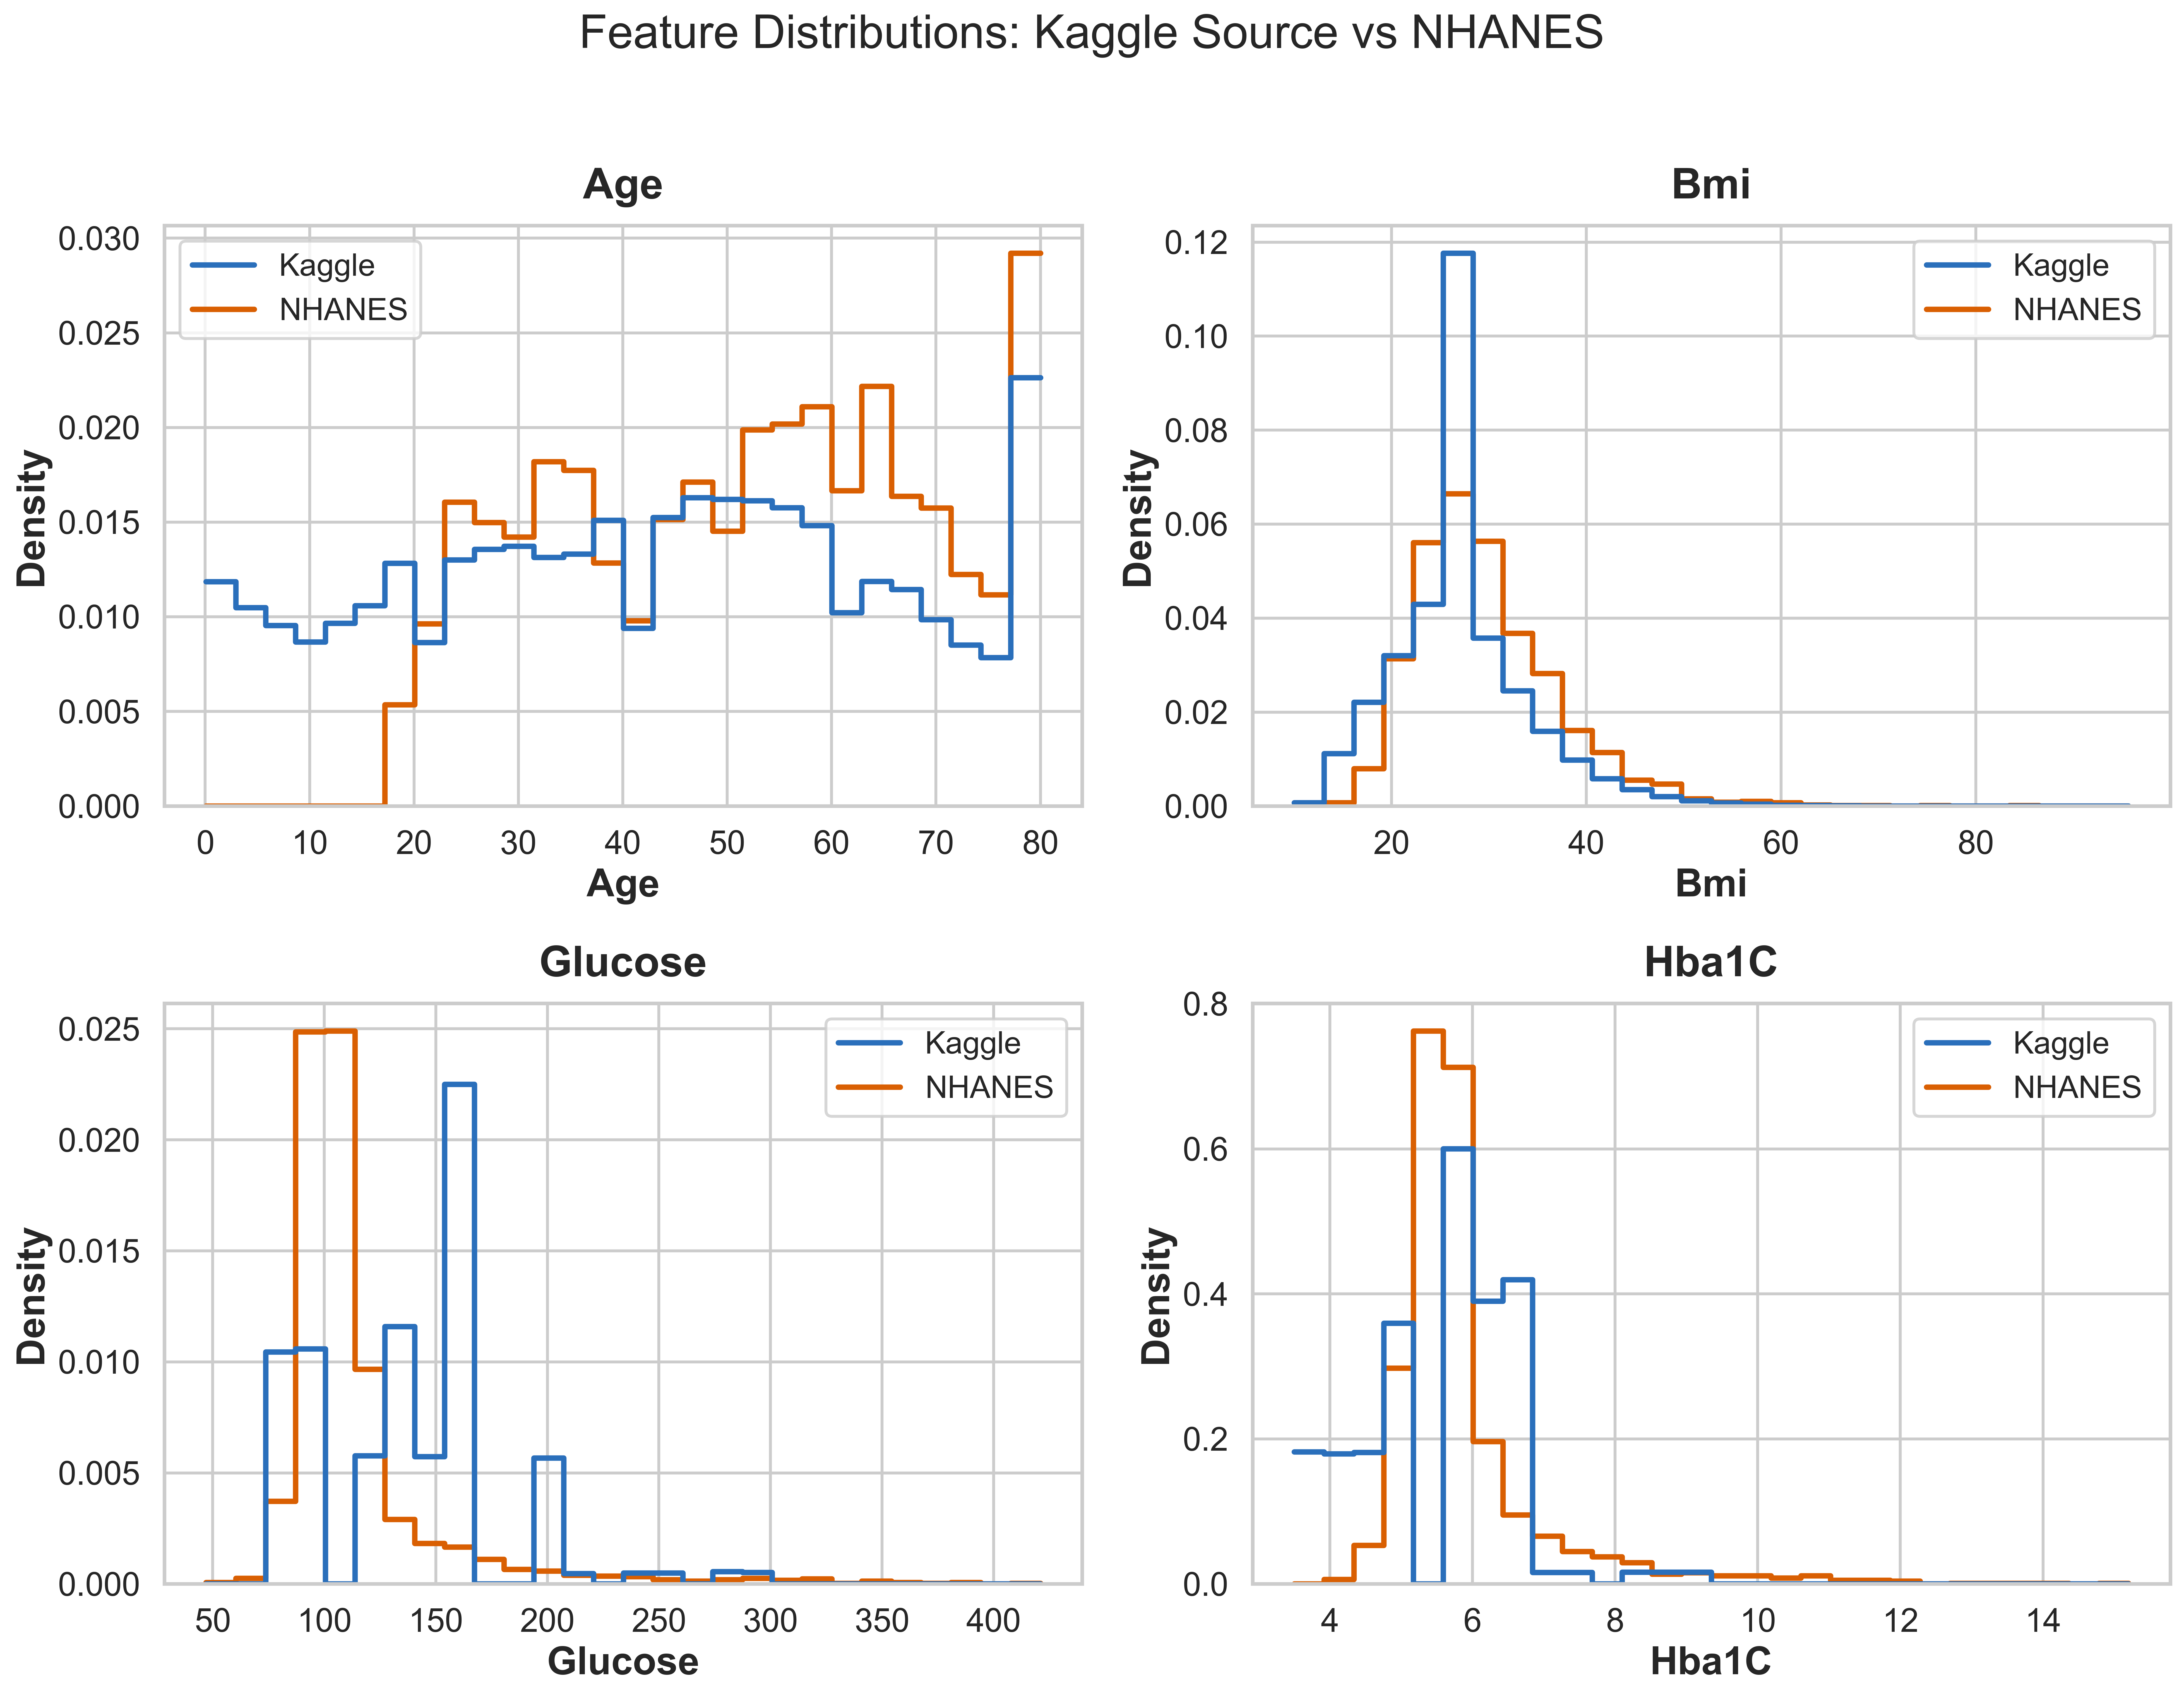
\includegraphics[width=0.95\linewidth]{figure_01a_feature_histograms_kaggle_vs_nhanes.png}
\caption{Feature distributions comparing the Kaggle source dataset with NHANES.}
\label{fig:hist_nhanes}
\end{figure}

\begin{figure}[H]
\centering
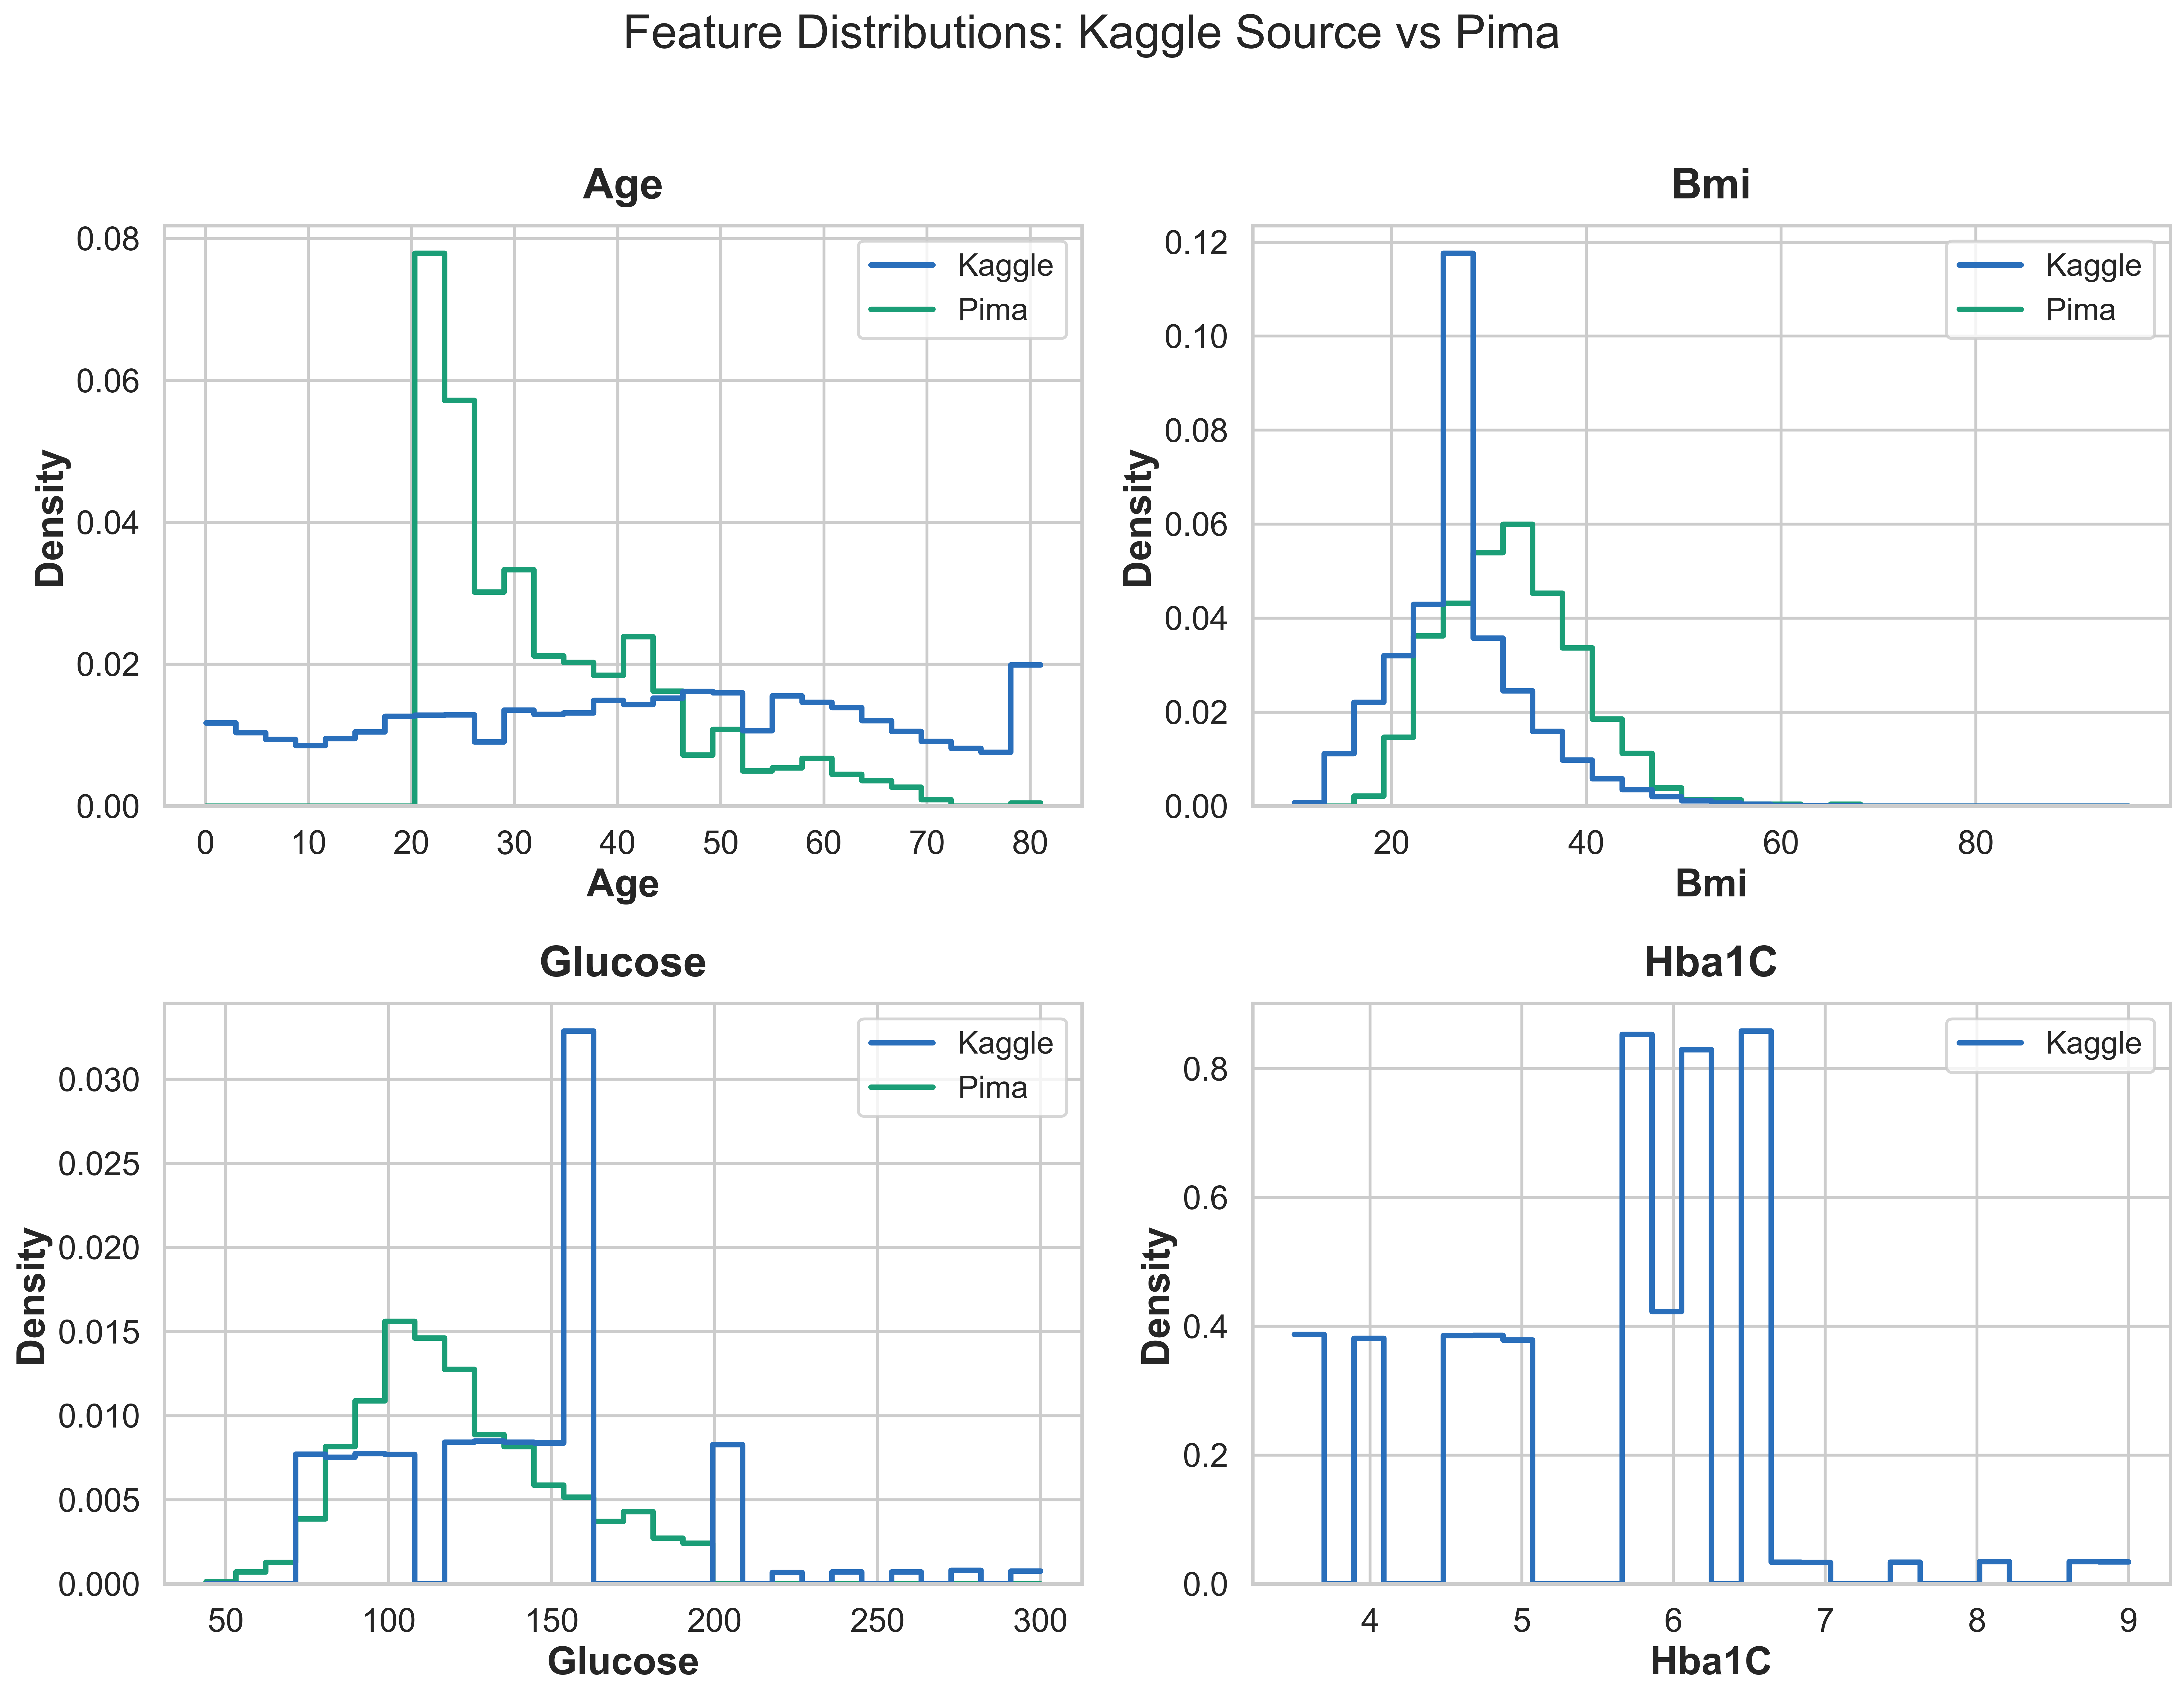
\includegraphics[width=0.95\linewidth]{figure_01b_feature_histograms_kaggle_vs_pima.png}
\caption{Feature distributions comparing the Kaggle source dataset with Pima.}
\label{fig:hist_pima}
\end{figure}

\begin{figure}[H]
\centering
\includegraphics[width=0.95\linewidth]{figure_02_low_dimensional_shift.png}
\caption{Low-dimensional visualization of dataset shift using PCA, t-SNE, and UMAP.}
\label{fig:lowdim}
\end{figure}

\subsection{Internal Source Performance}
Table~\ref{tab:internal} reports internal source test performance for all 15 source models. CatBoost with routine or extended clinical features achieved the highest ROC-AUC, 0.977, with ECE 0.006. XGBoost was nearly identical. Screening-only models had much weaker discrimination, showing the importance of glucose and HbA1c.

\begin{landscape}
\begin{longtable}{llrrrrrrr}
\caption{Internal source test performance for all five model families and three feature sets.}
\label{tab:internal}\\
\toprule
Feature set & Model & Accuracy & ROC-AUC & PR-AUC & Sens. & Spec. & Brier & ECE \\
\midrule
\endfirsthead
\toprule
Feature set & Model & Accuracy & ROC-AUC & PR-AUC & Sens. & Spec. & Brier & ECE \\
\midrule
\endhead
Screening & Logistic regression & 0.724 & 0.823 & 0.304 & 0.784 & 0.718 & 0.178 & 0.276 \\
Screening & Random forest & 0.731 & 0.821 & 0.294 & 0.765 & 0.728 & 0.161 & 0.250 \\
Screening & XGBoost & 0.911 & 0.823 & 0.306 & 0.058 & 0.994 & 0.070 & 0.007 \\
Screening & LightGBM & 0.734 & 0.816 & 0.301 & 0.747 & 0.732 & 0.166 & 0.240 \\
Screening & CatBoost & 0.911 & 0.825 & 0.304 & 0.056 & 0.994 & 0.070 & 0.005 \\
Routine clinical & Logistic regression & 0.886 & 0.960 & 0.812 & 0.876 & 0.886 & 0.080 & 0.127 \\
Routine clinical & Random forest & 0.903 & 0.974 & 0.874 & 0.901 & 0.904 & 0.062 & 0.130 \\
Routine clinical & XGBoost & 0.971 & 0.977 & 0.880 & 0.699 & 0.997 & 0.024 & 0.007 \\
Routine clinical & LightGBM & 0.925 & 0.975 & 0.876 & 0.863 & 0.931 & 0.048 & 0.064 \\
Routine clinical & CatBoost & 0.971 & 0.977 & 0.880 & 0.696 & 0.997 & 0.024 & 0.006 \\
Extended transport & Logistic regression & 0.886 & 0.960 & 0.812 & 0.876 & 0.886 & 0.080 & 0.127 \\
Extended transport & Random forest & 0.904 & 0.974 & 0.874 & 0.896 & 0.905 & 0.061 & 0.128 \\
Extended transport & XGBoost & 0.971 & 0.977 & 0.879 & 0.700 & 0.997 & 0.024 & 0.007 \\
Extended transport & LightGBM & 0.925 & 0.975 & 0.876 & 0.863 & 0.931 & 0.048 & 0.064 \\
Extended transport & CatBoost & 0.971 & 0.977 & 0.880 & 0.696 & 0.997 & 0.024 & 0.006 \\
\bottomrule
\end{longtable}
\end{landscape}

\begin{figure}[H]
\centering
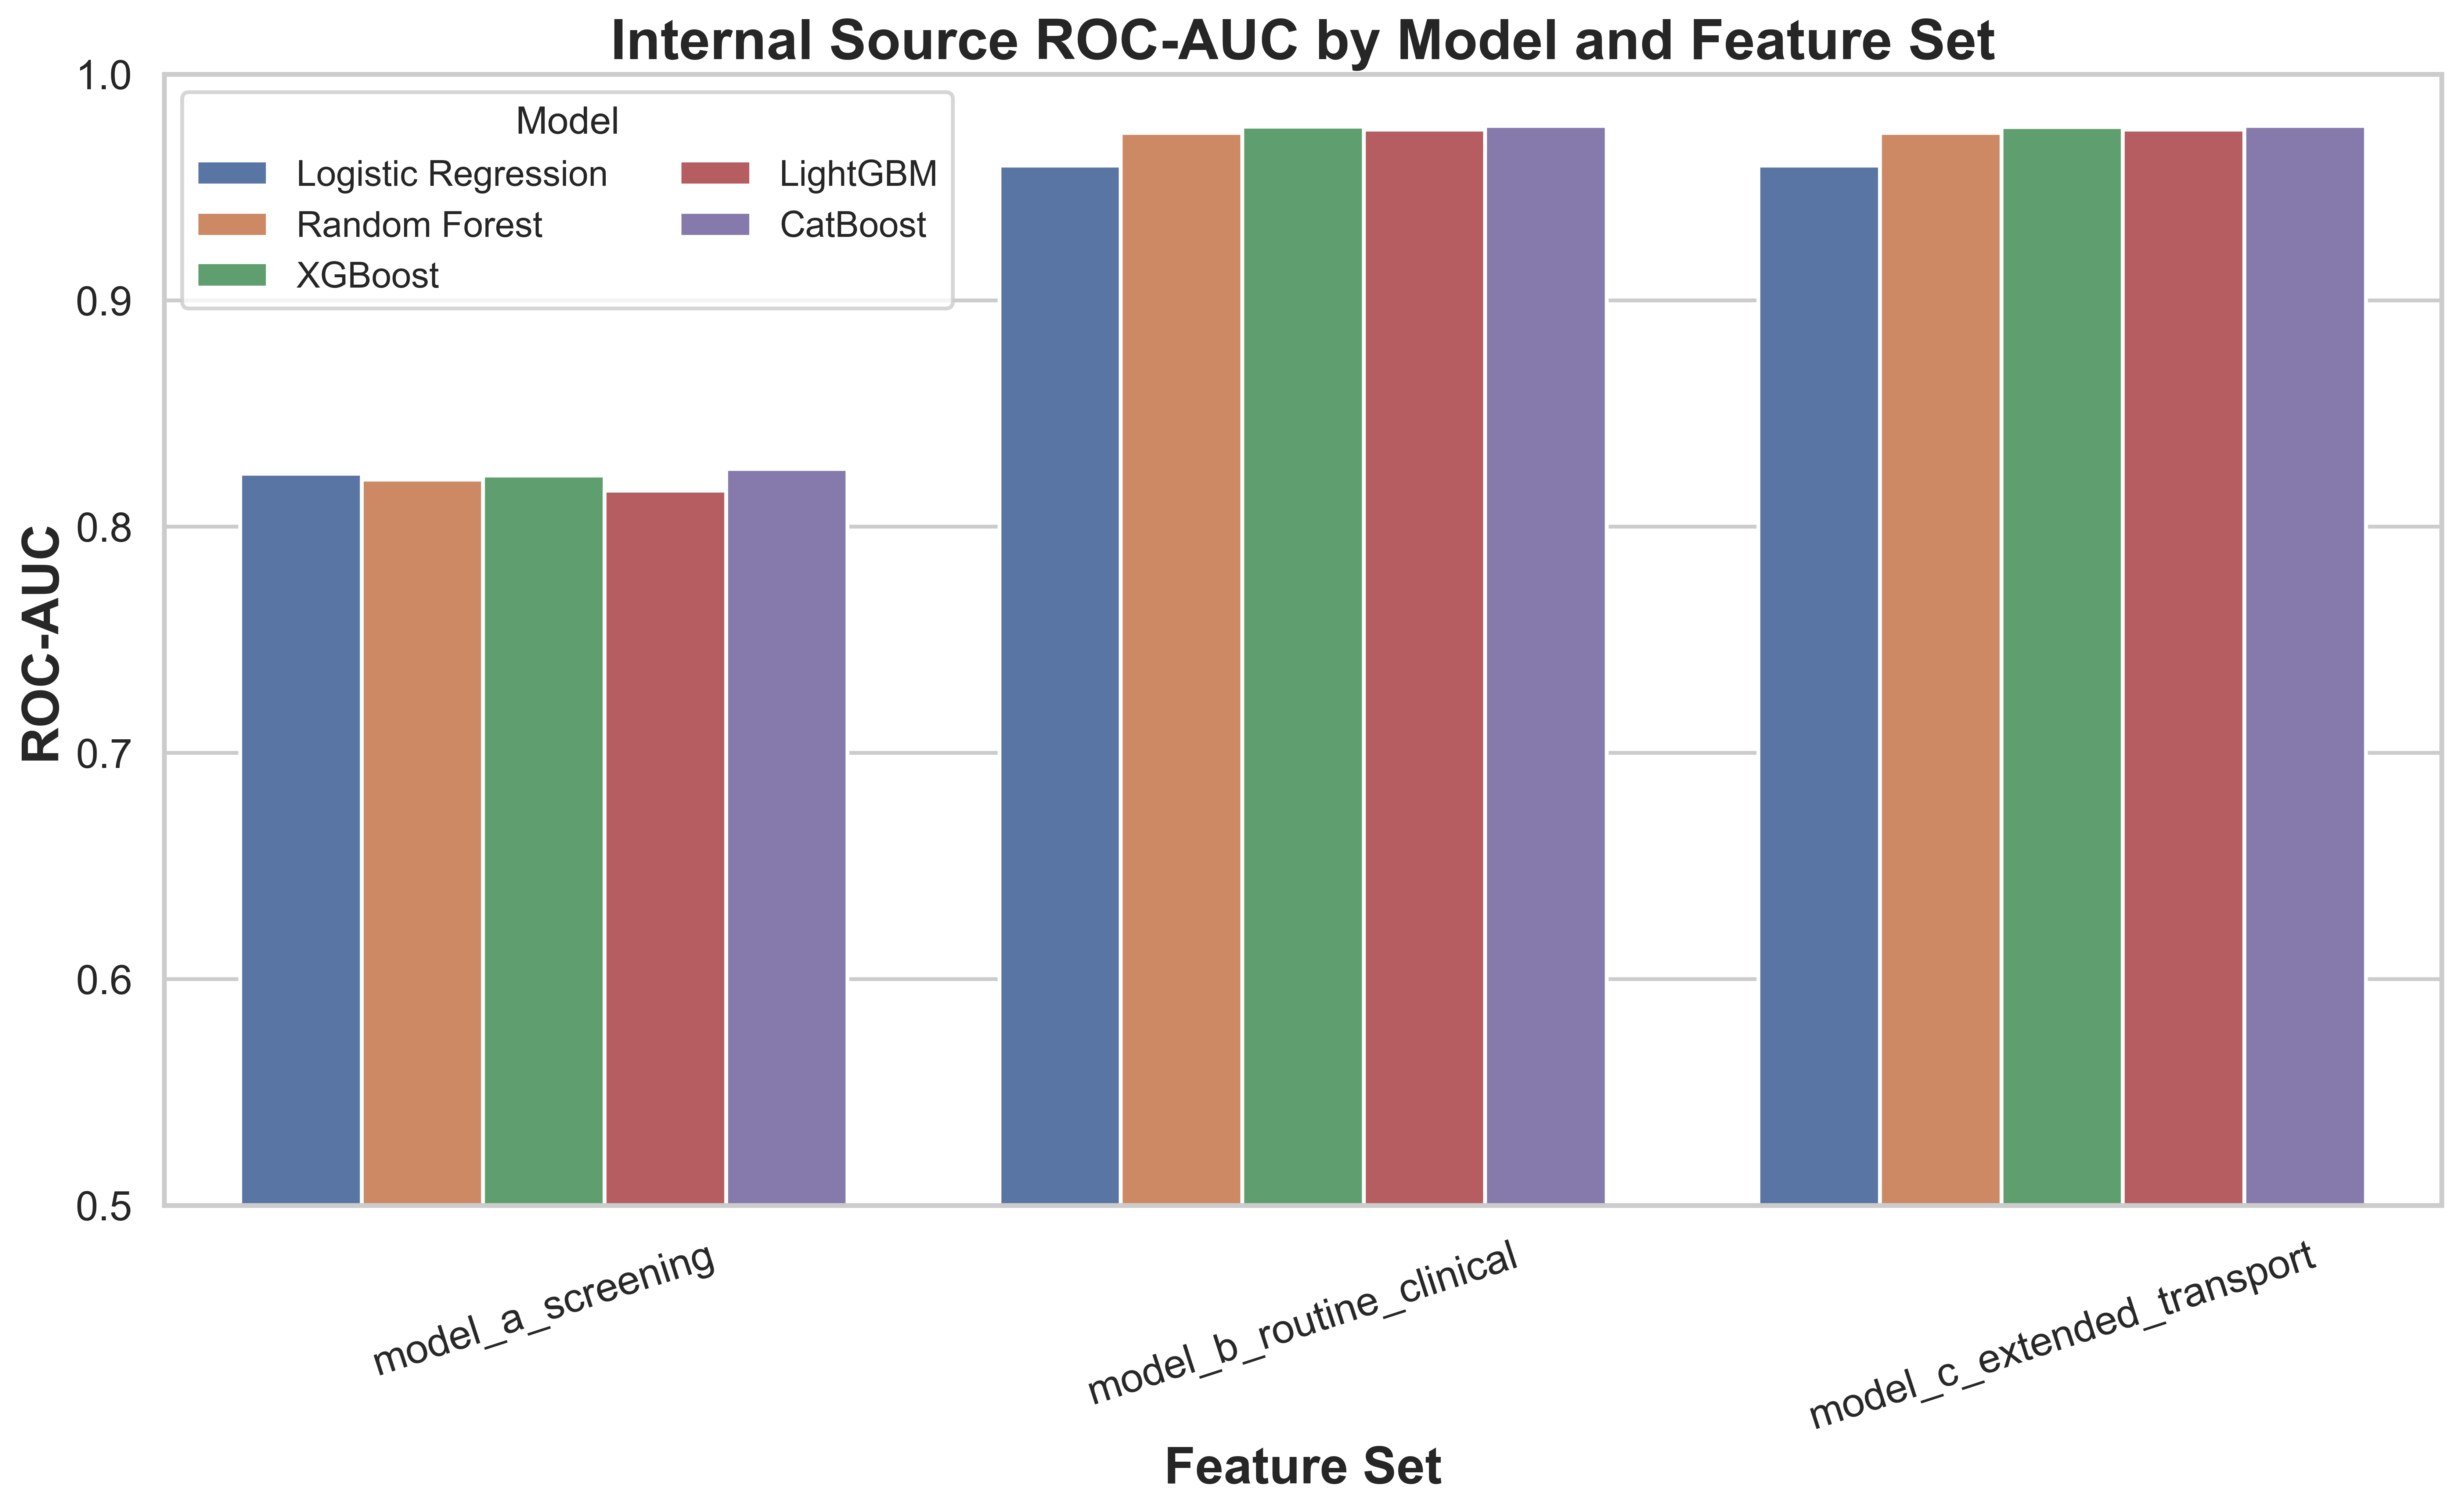
\includegraphics[width=0.95\linewidth]{figure_03_internal_model_comparison.png}
\caption{Internal source ROC-AUC by feature set and model family.}
\label{fig:internal_model}
\end{figure}

\subsection{Calibration Results}
The best calibration method differed by feature set and model. For screening models, beta calibration and isotonic regression were often best. For routine and extended clinical models, uncalibrated probabilities, temperature scaling, and isotonic regression were competitive depending on the model.

\begin{longtable}{lllrr}
\caption{Best calibration method by feature set and model.}
\label{tab:calibration}\\
\toprule
Feature set & Model & Best method & Mean ECE & Mean Brier \\
\midrule
\endfirsthead
\toprule
Feature set & Model & Best method & Mean ECE & Mean Brier \\
\midrule
\endhead
Screening & Logistic regression & Beta & 0.089 & 0.155 \\
Screening & Random forest & Isotonic & 0.099 & 0.161 \\
Screening & XGBoost & Beta & 0.096 & 0.160 \\
Screening & LightGBM & Beta & 0.097 & 0.160 \\
Screening & CatBoost & Beta & 0.096 & 0.161 \\
Routine clinical & Logistic regression & Uncalibrated & 0.105 & 0.113 \\
Routine clinical & Random forest & Uncalibrated & 0.112 & 0.117 \\
Routine clinical & XGBoost & Temperature & 0.128 & 0.135 \\
Routine clinical & LightGBM & Temperature & 0.116 & 0.122 \\
Routine clinical & CatBoost & Isotonic & 0.120 & 0.132 \\
Extended transport & Logistic regression & Uncalibrated & 0.105 & 0.113 \\
Extended transport & Random forest & Uncalibrated & 0.111 & 0.116 \\
Extended transport & XGBoost & Temperature & 0.129 & 0.135 \\
Extended transport & LightGBM & Temperature & 0.116 & 0.122 \\
Extended transport & CatBoost & Isotonic & 0.120 & 0.132 \\
\bottomrule
\end{longtable}

\subsection{NHANES External Validation}
NHANES was the primary external validation dataset. The best external ROC-AUC was 0.943 using logistic regression with routine or extended features. Adaptive calibration often improved ECE while preserving useful discrimination. Table~\ref{tab:nhanes_adaptive} reports adaptive calibration results in NHANES.

\begin{landscape}
\begin{longtable}{llrrrrrrr}
\caption{NHANES adaptive calibration results, sorted by ROC-AUC within the target dataset.}
\label{tab:nhanes_adaptive}\\
\toprule
Feature set & Model & ROC-AUC & PR-AUC & Accuracy & Sens. & Spec. & Brier & ECE \\
\midrule
\endfirsthead
\toprule
Feature set & Model & ROC-AUC & PR-AUC & Accuracy & Sens. & Spec. & Brier & ECE \\
\midrule
\endhead
Routine clinical & Logistic regression & 0.939 & 0.778 & 0.909 & 0.634 & 0.968 & 0.067 & 0.019 \\
Extended transport & Logistic regression & 0.939 & 0.778 & 0.909 & 0.634 & 0.968 & 0.067 & 0.019 \\
Extended transport & Random forest & 0.924 & 0.729 & 0.904 & 0.535 & 0.983 & 0.073 & 0.018 \\
Routine clinical & LightGBM & 0.923 & 0.734 & 0.908 & 0.564 & 0.981 & 0.072 & 0.015 \\
Extended transport & LightGBM & 0.923 & 0.734 & 0.908 & 0.564 & 0.981 & 0.072 & 0.015 \\
Routine clinical & XGBoost & 0.923 & 0.739 & 0.911 & 0.693 & 0.958 & 0.069 & 0.017 \\
Routine clinical & Random forest & 0.923 & 0.727 & 0.906 & 0.545 & 0.983 & 0.073 & 0.017 \\
Extended transport & XGBoost & 0.922 & 0.740 & 0.911 & 0.688 & 0.959 & 0.070 & 0.012 \\
Routine clinical & CatBoost & 0.918 & 0.744 & 0.906 & 0.559 & 0.980 & 0.073 & 0.013 \\
Extended transport & CatBoost & 0.918 & 0.744 & 0.906 & 0.559 & 0.980 & 0.073 & 0.013 \\
Screening & Random forest & 0.783 & 0.375 & 0.823 & 0.064 & 0.985 & 0.124 & 0.022 \\
Screening & LightGBM & 0.774 & 0.372 & 0.827 & 0.109 & 0.981 & 0.125 & 0.008 \\
Screening & Logistic regression & 0.773 & 0.370 & 0.827 & 0.035 & 0.997 & 0.125 & 0.015 \\
Screening & XGBoost & 0.767 & 0.369 & 0.827 & 0.089 & 0.985 & 0.126 & 0.007 \\
Screening & CatBoost & 0.762 & 0.357 & 0.829 & 0.089 & 0.987 & 0.127 & 0.013 \\
\bottomrule
\end{longtable}
\end{landscape}

\subsection{Pima Stress-Test Results}
Pima was harder than NHANES. The best Pima ROC-AUC was 0.806 with logistic regression, but coverage remained poor. Table~\ref{tab:pima_adaptive} reports adaptive calibration results in Pima.

\begin{landscape}
\begin{longtable}{llrrrrrrr}
\caption{Pima adaptive calibration results.}
\label{tab:pima_adaptive}\\
\toprule
Feature set & Model & ROC-AUC & PR-AUC & Accuracy & Sens. & Spec. & Brier & ECE \\
\midrule
\endfirsthead
\toprule
Feature set & Model & ROC-AUC & PR-AUC & Accuracy & Sens. & Spec. & Brier & ECE \\
\midrule
\endhead
Routine clinical & Logistic regression & 0.802 & 0.618 & 0.740 & 0.575 & 0.828 & 0.172 & 0.044 \\
Extended transport & Logistic regression & 0.802 & 0.618 & 0.740 & 0.575 & 0.828 & 0.172 & 0.044 \\
Routine clinical & Random forest & 0.791 & 0.584 & 0.716 & 0.500 & 0.832 & 0.179 & 0.075 \\
Extended transport & Random forest & 0.787 & 0.578 & 0.721 & 0.567 & 0.804 & 0.179 & 0.039 \\
Routine clinical & LightGBM & 0.775 & 0.583 & 0.706 & 0.381 & 0.880 & 0.183 & 0.074 \\
Extended transport & LightGBM & 0.775 & 0.583 & 0.706 & 0.381 & 0.880 & 0.183 & 0.074 \\
Routine clinical & CatBoost & 0.769 & 0.563 & 0.716 & 0.485 & 0.840 & 0.183 & 0.032 \\
Extended transport & CatBoost & 0.769 & 0.563 & 0.716 & 0.485 & 0.840 & 0.183 & 0.032 \\
Extended transport & XGBoost & 0.762 & 0.571 & 0.745 & 0.604 & 0.820 & 0.185 & 0.078 \\
Routine clinical & XGBoost & 0.758 & 0.555 & 0.734 & 0.597 & 0.808 & 0.187 & 0.044 \\
Screening & Random forest & 0.710 & 0.480 & 0.667 & 0.321 & 0.852 & 0.202 & 0.073 \\
Screening & Logistic regression & 0.698 & 0.478 & 0.646 & 0.299 & 0.832 & 0.208 & 0.094 \\
Screening & XGBoost & 0.693 & 0.468 & 0.646 & 0.306 & 0.828 & 0.205 & 0.065 \\
Screening & CatBoost & 0.690 & 0.465 & 0.646 & 0.284 & 0.840 & 0.205 & 0.069 \\
Screening & LightGBM & 0.680 & 0.484 & 0.661 & 0.433 & 0.784 & 0.210 & 0.064 \\
\bottomrule
\end{longtable}
\end{landscape}

\subsection{Conformal Prediction}
In NHANES, the best 90\% ATCP coverage was 0.911, close to the nominal target. In Pima, the best 90\% ATCP coverage was only 0.747. This shows that adaptive conformal recalibration was useful in NHANES but not sufficient under the more severe Pima shift.

\begin{table}[H]
\centering
\caption{Best 90\% ATCP coverage by target dataset.}
\label{tab:atcp}
\begin{adjustbox}{width=\textwidth}
\begin{tabular}{llllrrrr}
\toprule
Target & Feature set & Model & Scenario & Coverage & Gap & Mean set size & Class-1 coverage \\
\midrule
NHANES & Routine clinical & Logistic regression & Adaptive isotonic & 0.911 & 0.011 & 1.003 & 0.644 \\
NHANES & Extended transport & Logistic regression & Adaptive isotonic & 0.911 & 0.011 & 1.003 & 0.644 \\
NHANES & Routine clinical & LightGBM & Adaptive isotonic & 0.907 & 0.007 & 0.999 & 0.559 \\
Pima & Routine clinical & Logistic regression & Naive transfer & 0.747 & -0.153 & 1.052 & 0.485 \\
Pima & Extended transport & Logistic regression & Naive transfer & 0.747 & -0.153 & 1.052 & 0.485 \\
Pima & Routine clinical & Logistic regression & Adaptive isotonic & 0.740 & -0.160 & 1.000 & 0.575 \\
\bottomrule
\end{tabular}
\end{adjustbox}
\end{table}

\begin{figure}[H]
\centering
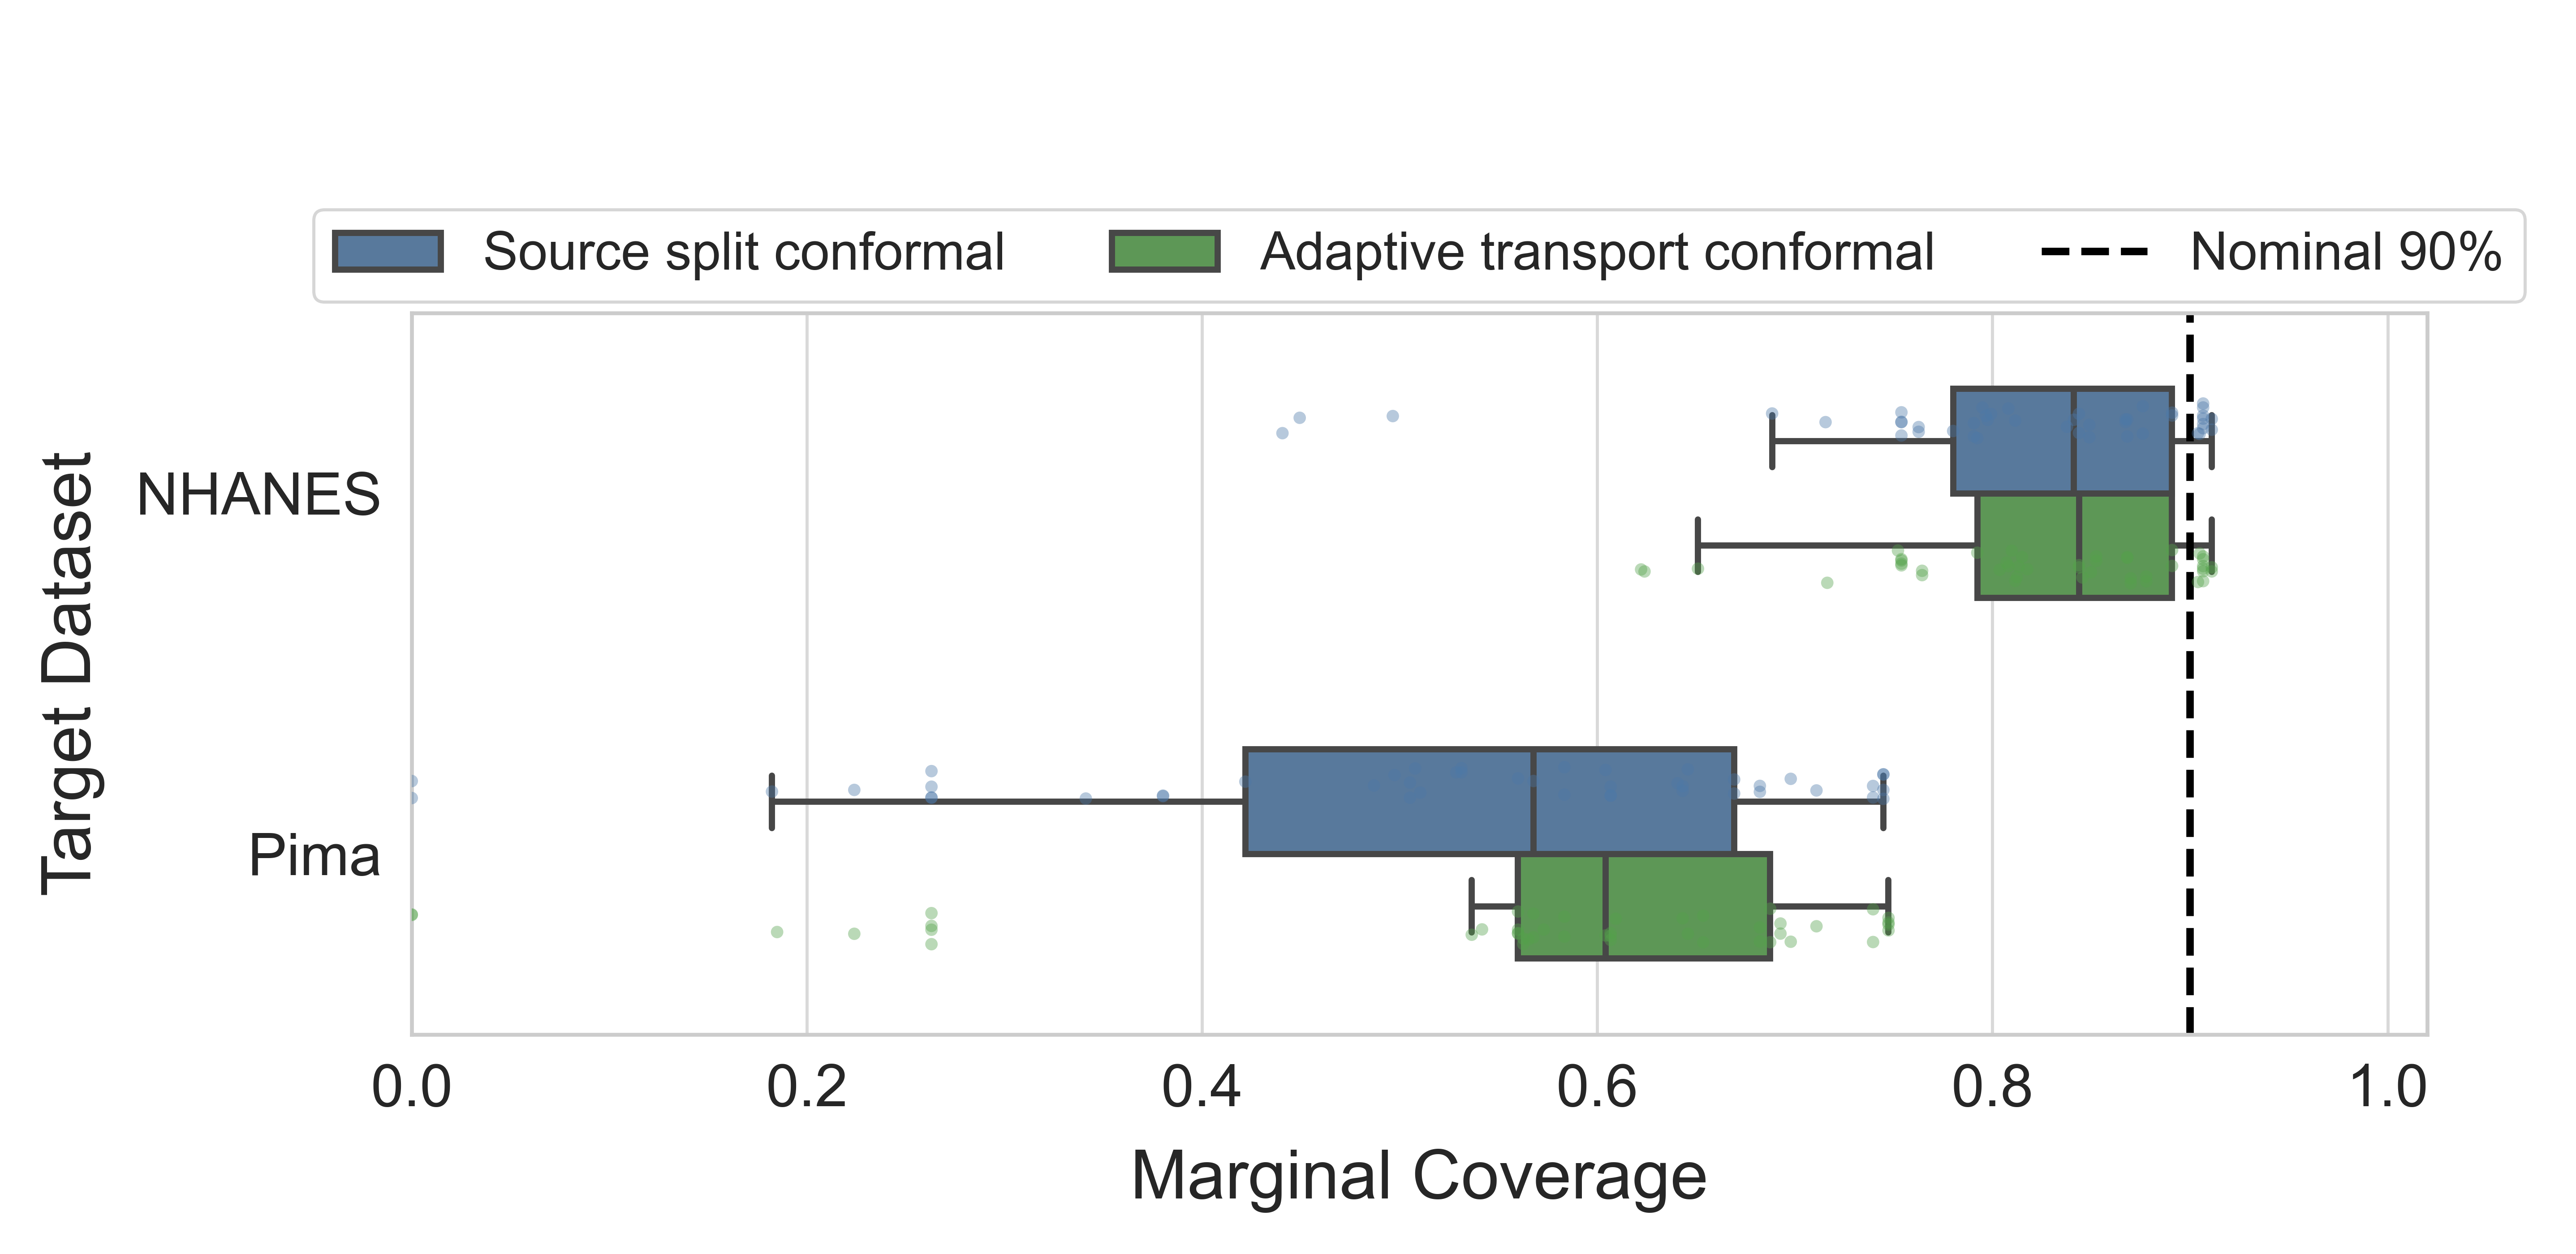
\includegraphics[width=0.95\linewidth]{figure_04_conformal_coverage.png}
\caption{External conformal coverage at 90\% confidence.}
\label{fig:conformal}
\end{figure}

\subsection{Transport Reliability Score}
The top TRS setting was NHANES with extended random forest and adaptive isotonic calibration. Its TRS was 0.737, with ROC-AUC 0.924, ECE 0.018, and ATCP coverage 0.904. LightGBM was competitive but did not rank first. The best Pima TRS was 0.670, much lower than the best NHANES TRS.

\begin{table}[H]
\centering
\caption{Top Transport Reliability Score settings.}
\label{tab:trs}
\begin{adjustbox}{width=\textwidth}
\begin{tabular}{llllrrrr}
\toprule
Target & Feature set & Model & Scenario & ROC-AUC & ECE & Coverage & TRS \\
\midrule
NHANES & Extended transport & Random forest & Adaptive isotonic & 0.924 & 0.018 & 0.904 & 0.737 \\
NHANES & Routine clinical & Random forest & Adaptive isotonic & 0.923 & 0.017 & 0.905 & 0.737 \\
NHANES & Extended transport & Logistic regression & Adaptive isotonic & 0.939 & 0.019 & 0.911 & 0.732 \\
NHANES & Routine clinical & Logistic regression & Adaptive isotonic & 0.939 & 0.019 & 0.911 & 0.732 \\
NHANES & Extended transport & LightGBM & Adaptive isotonic & 0.923 & 0.015 & 0.907 & 0.732 \\
NHANES & Routine clinical & LightGBM & Adaptive isotonic & 0.923 & 0.015 & 0.907 & 0.732 \\
Pima & Extended transport & Logistic regression & Adaptive isotonic & 0.802 & 0.044 & 0.740 & 0.670 \\
Pima & Routine clinical & Logistic regression & Adaptive isotonic & 0.802 & 0.044 & 0.740 & 0.670 \\
\bottomrule
\end{tabular}
\end{adjustbox}
\end{table}

\begin{figure}[H]
\centering

\includegraphics[width=0.95\linewidth]{figure_05_transport_reliability_score.png}
\caption{Transport Reliability Score rankings across target datasets.}
\label{fig:trs_all}
\end{figure}

\begin{figure}[H]
\centering
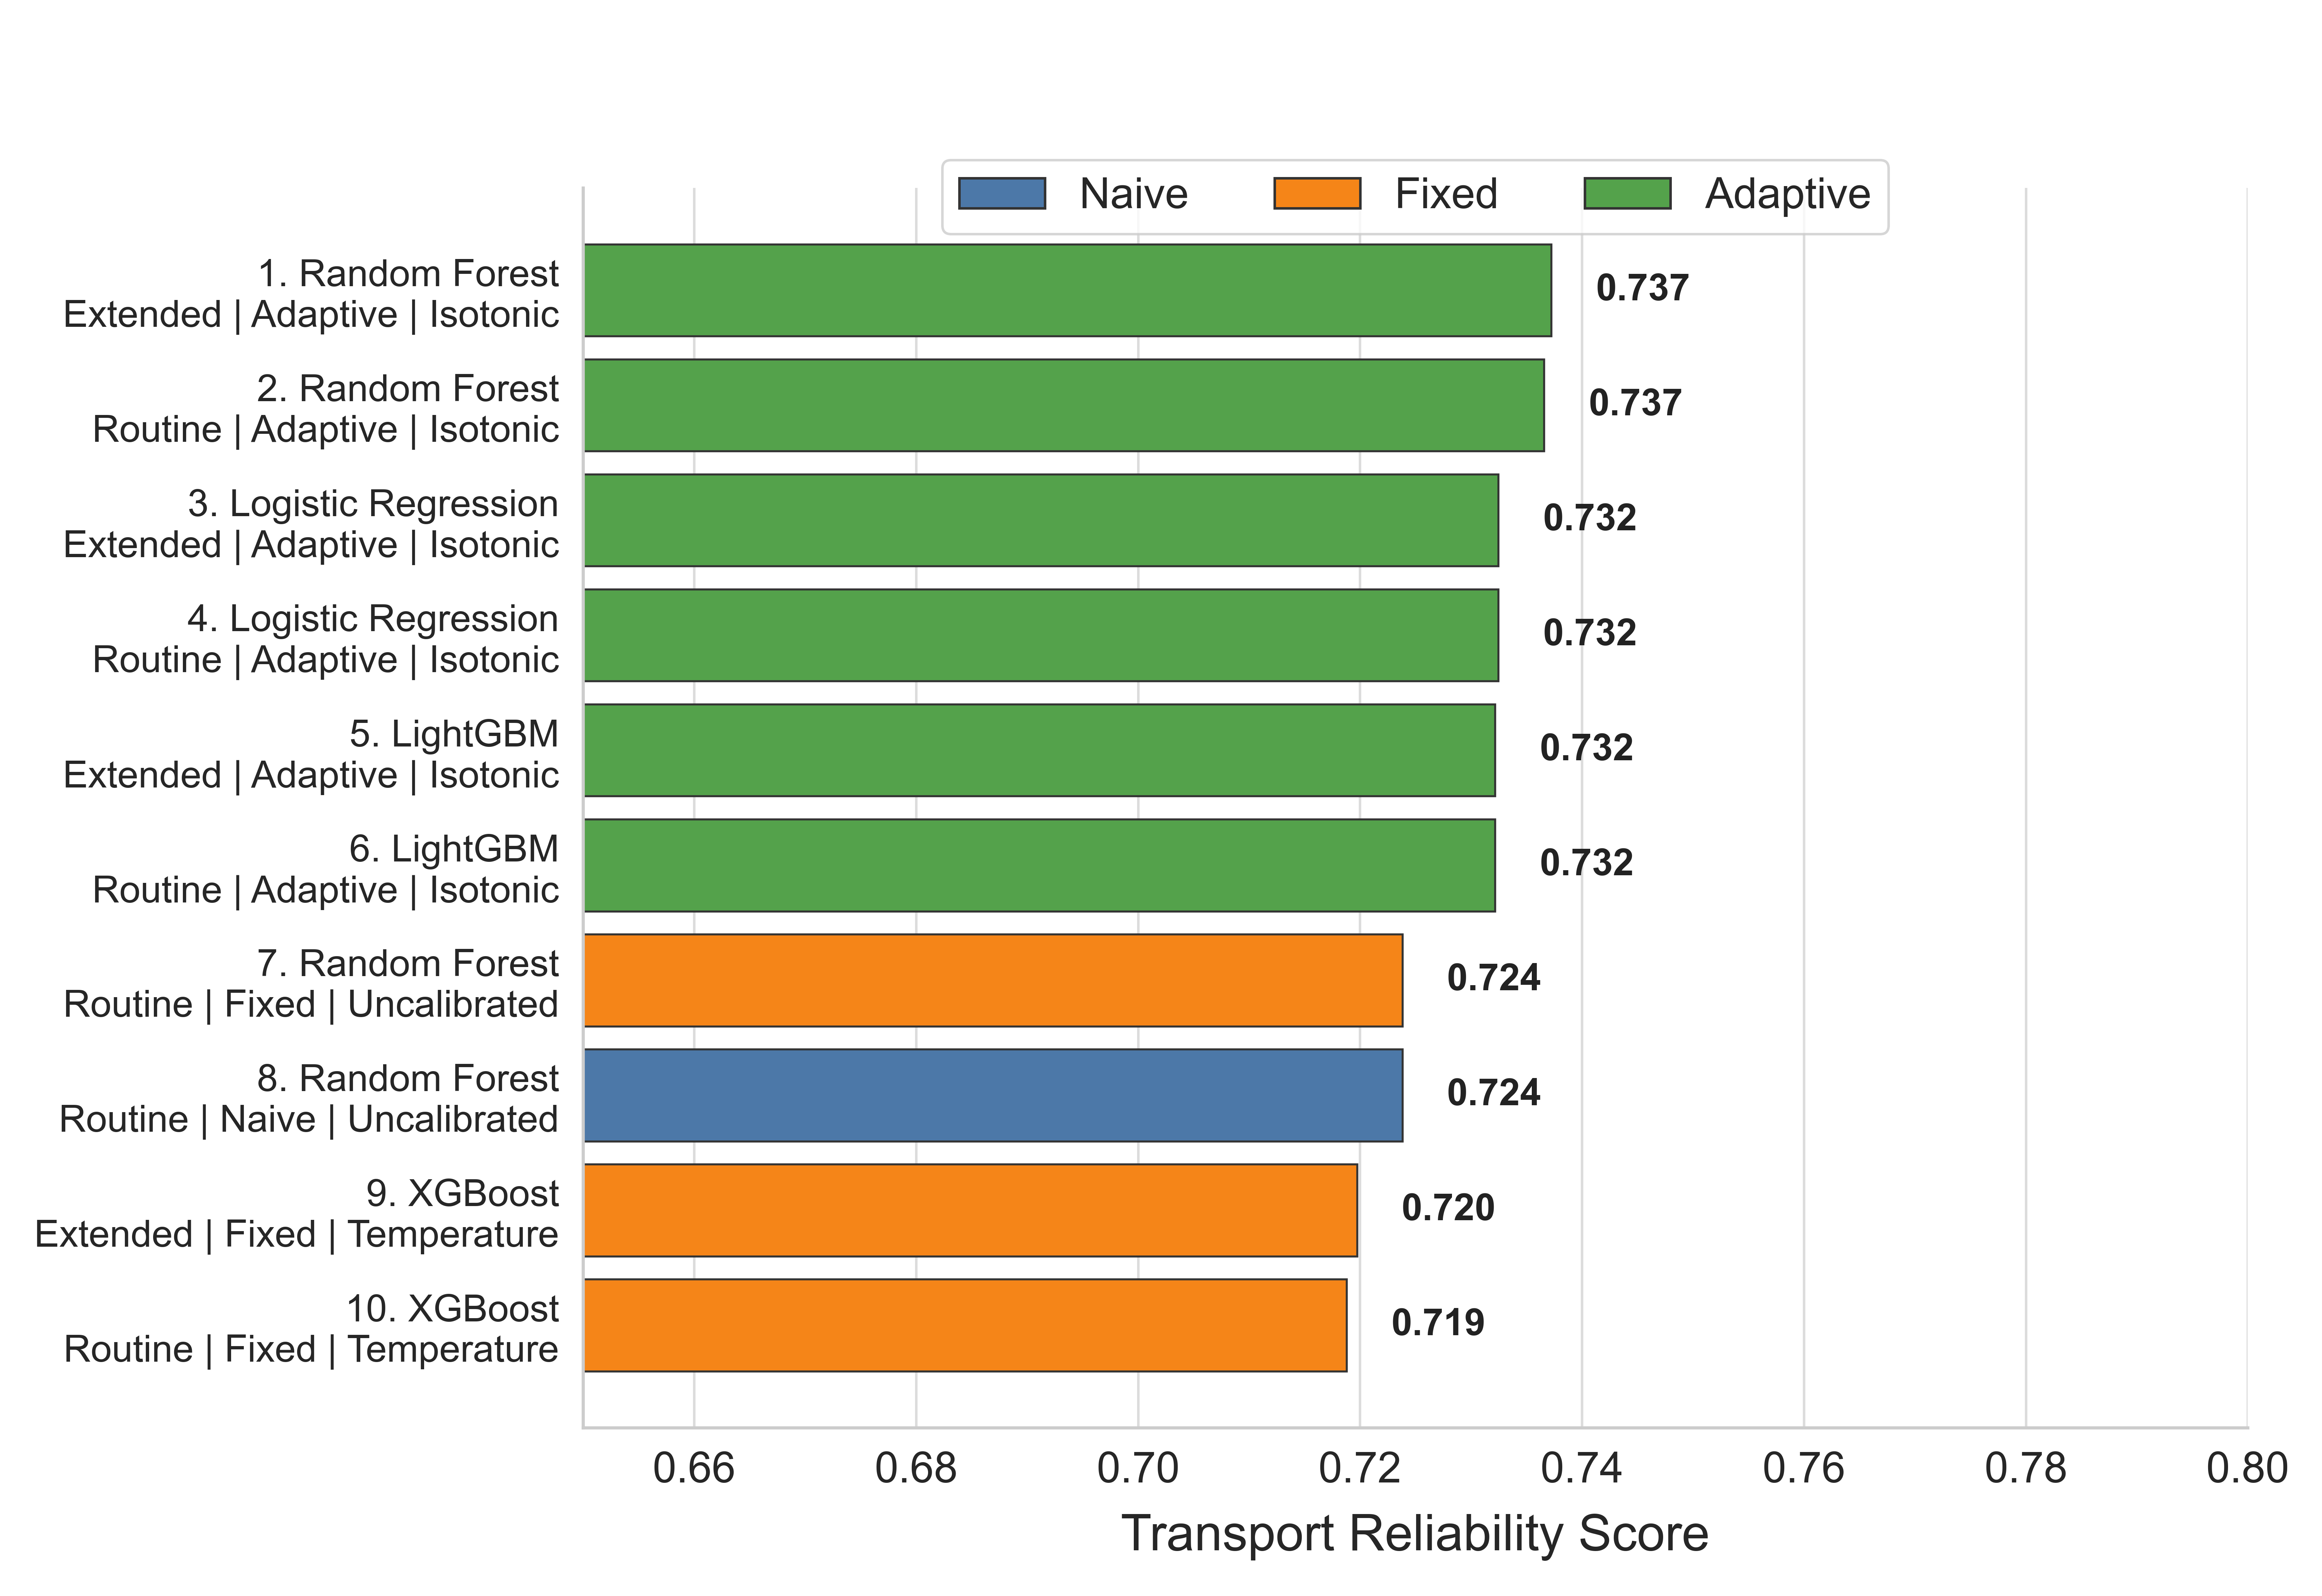
\includegraphics[width=0.95\linewidth]{figure_05_nhanes_transport_reliability_score.png}
\caption{NHANES Transport Reliability Score rankings.}
\label{fig:trs_nhanes}
\end{figure}

\begin{figure}[H]
\centering
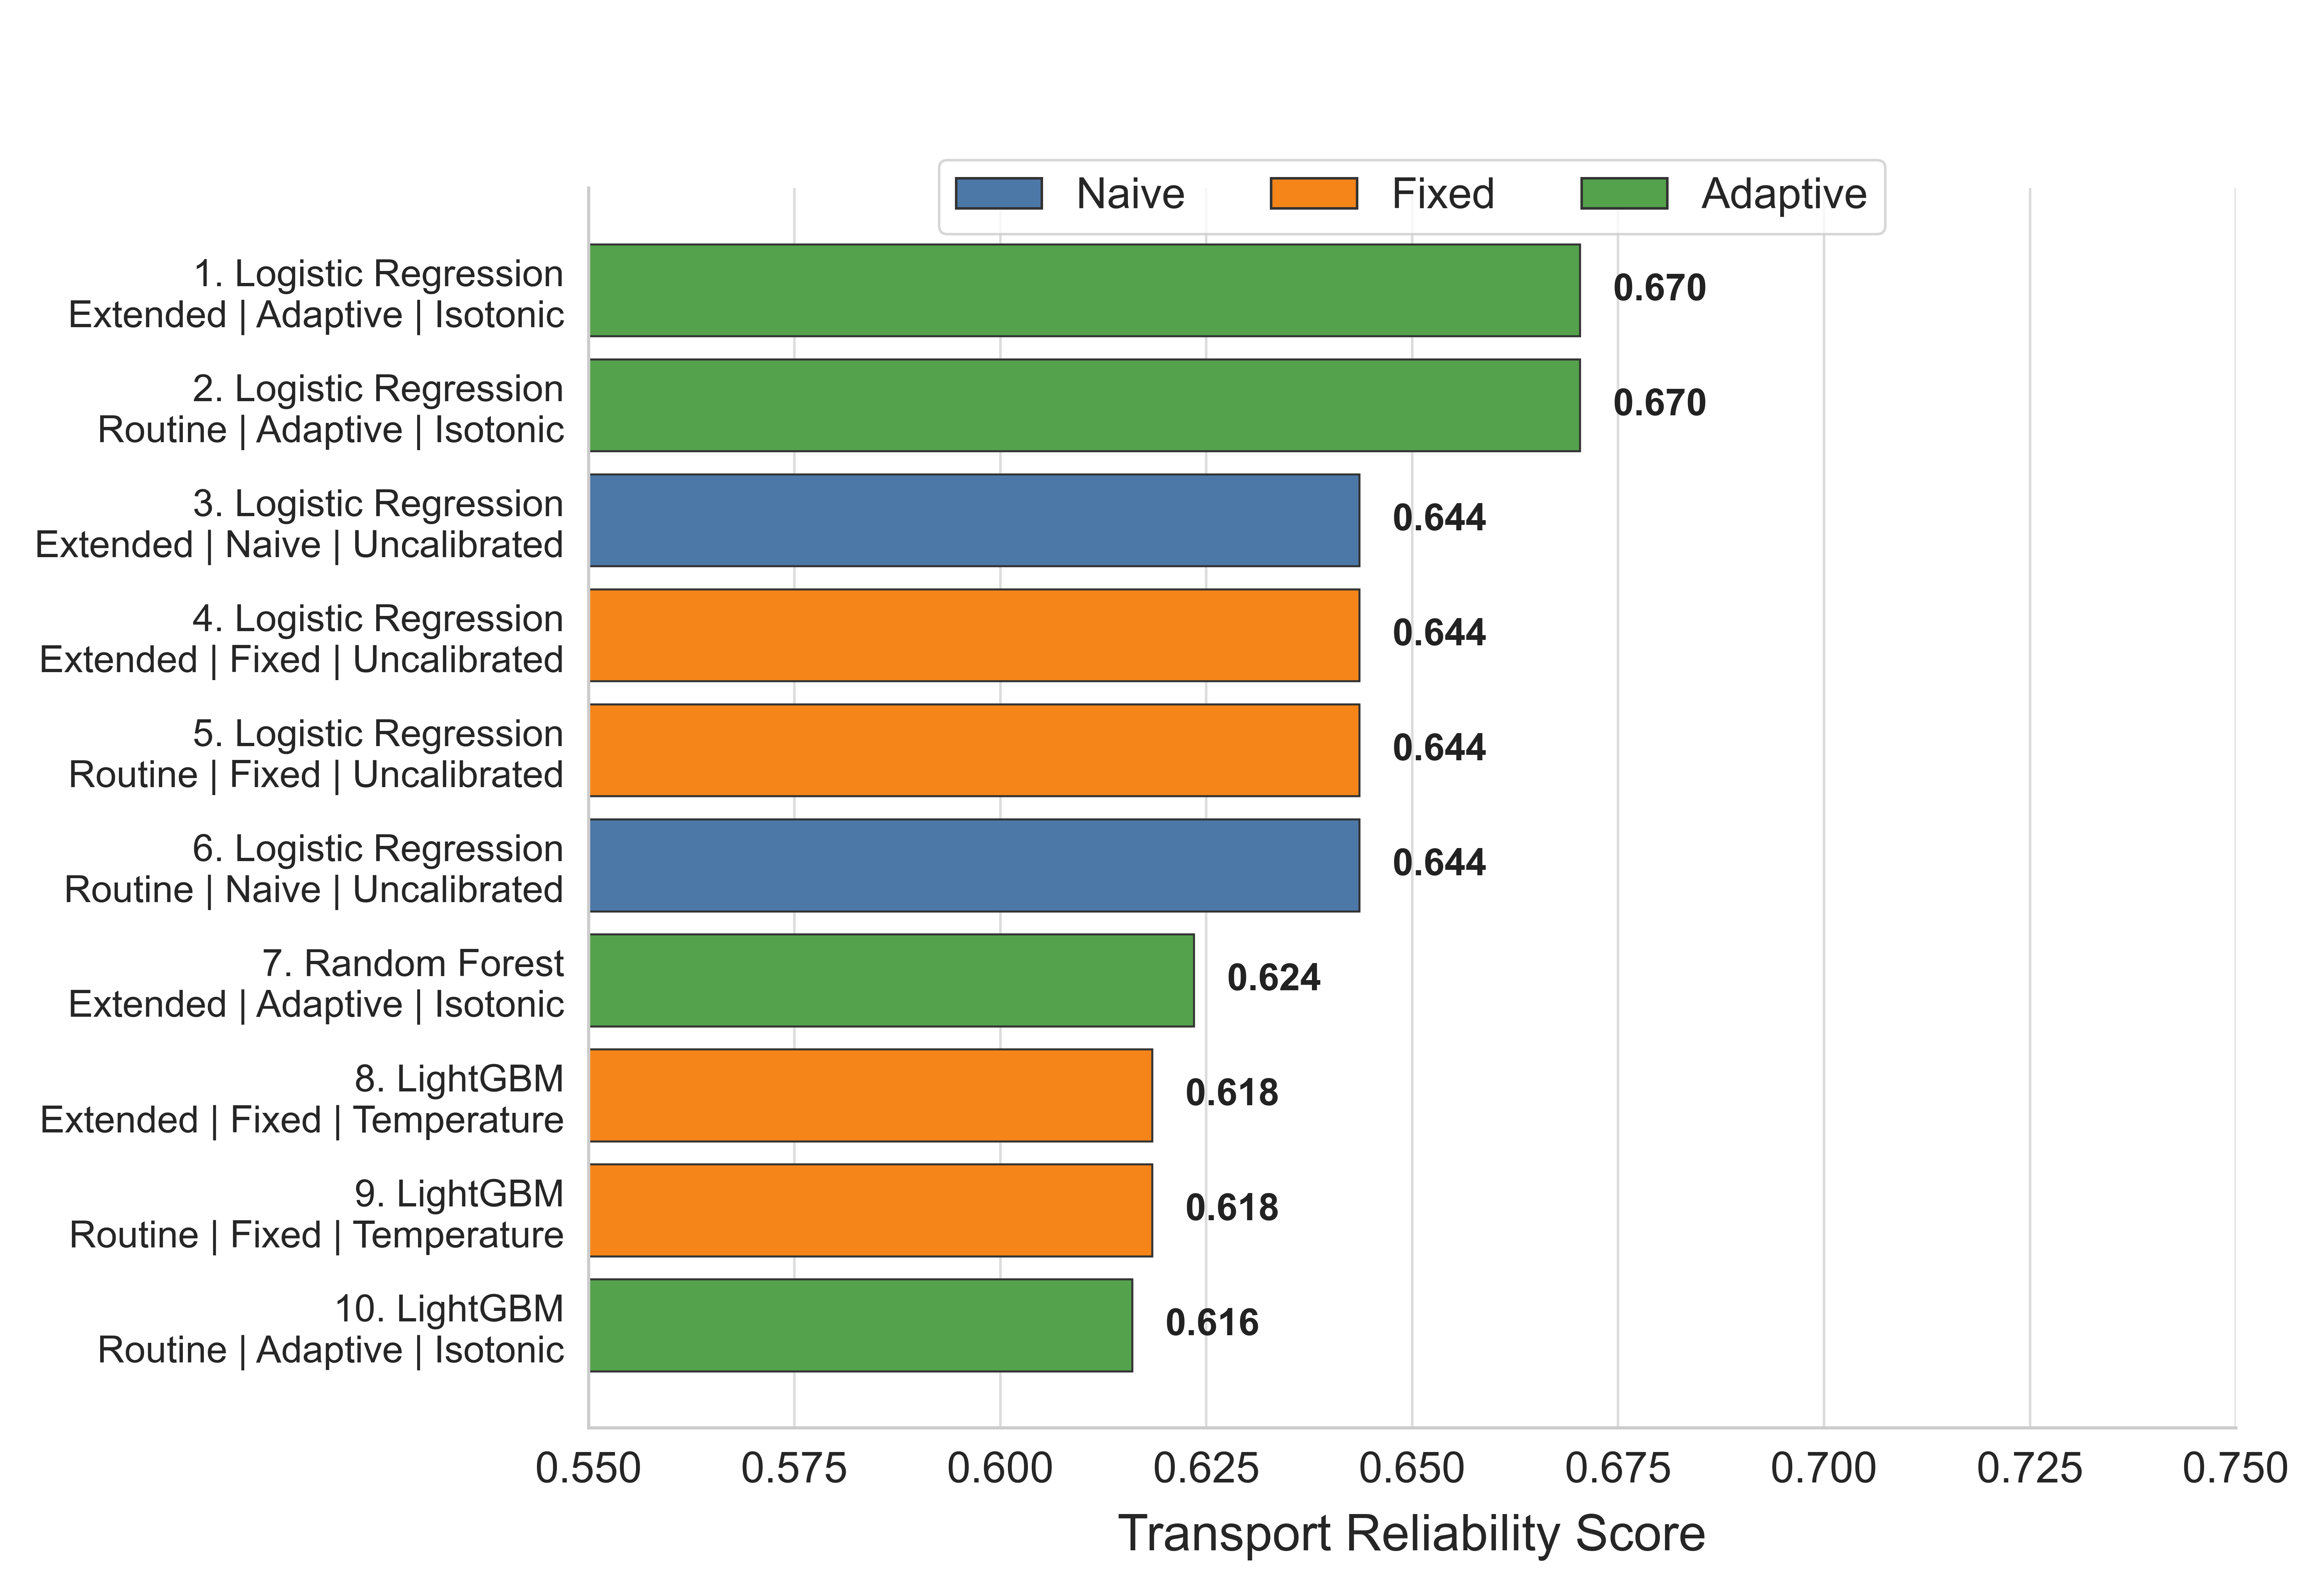
\includegraphics[width=0.95\linewidth]{figure_05_pima_transport_reliability_score.png}
\caption{Pima Transport Reliability Score rankings.}
\label{fig:trs_pima}
\end{figure}

\subsection{Reliability Diagrams and Bootstrap Intervals}
Reliability diagrams for NHANES show the effect of adaptive calibration. Bootstrap confidence intervals used 1,000 repeats. For the top TRS setting, the bootstrap estimate for ROC-AUC was 0.924 with 95\% CI 0.904--0.943; Brier score was 0.073 with 95\% CI 0.064--0.083; ECE was 0.023 with 95\% CI 0.013--0.034; and coverage was 0.904 with 95\% CI 0.890--0.918.

\begin{figure}[H]
\centering
\begin{subfigure}{0.48\linewidth}
    \centering
    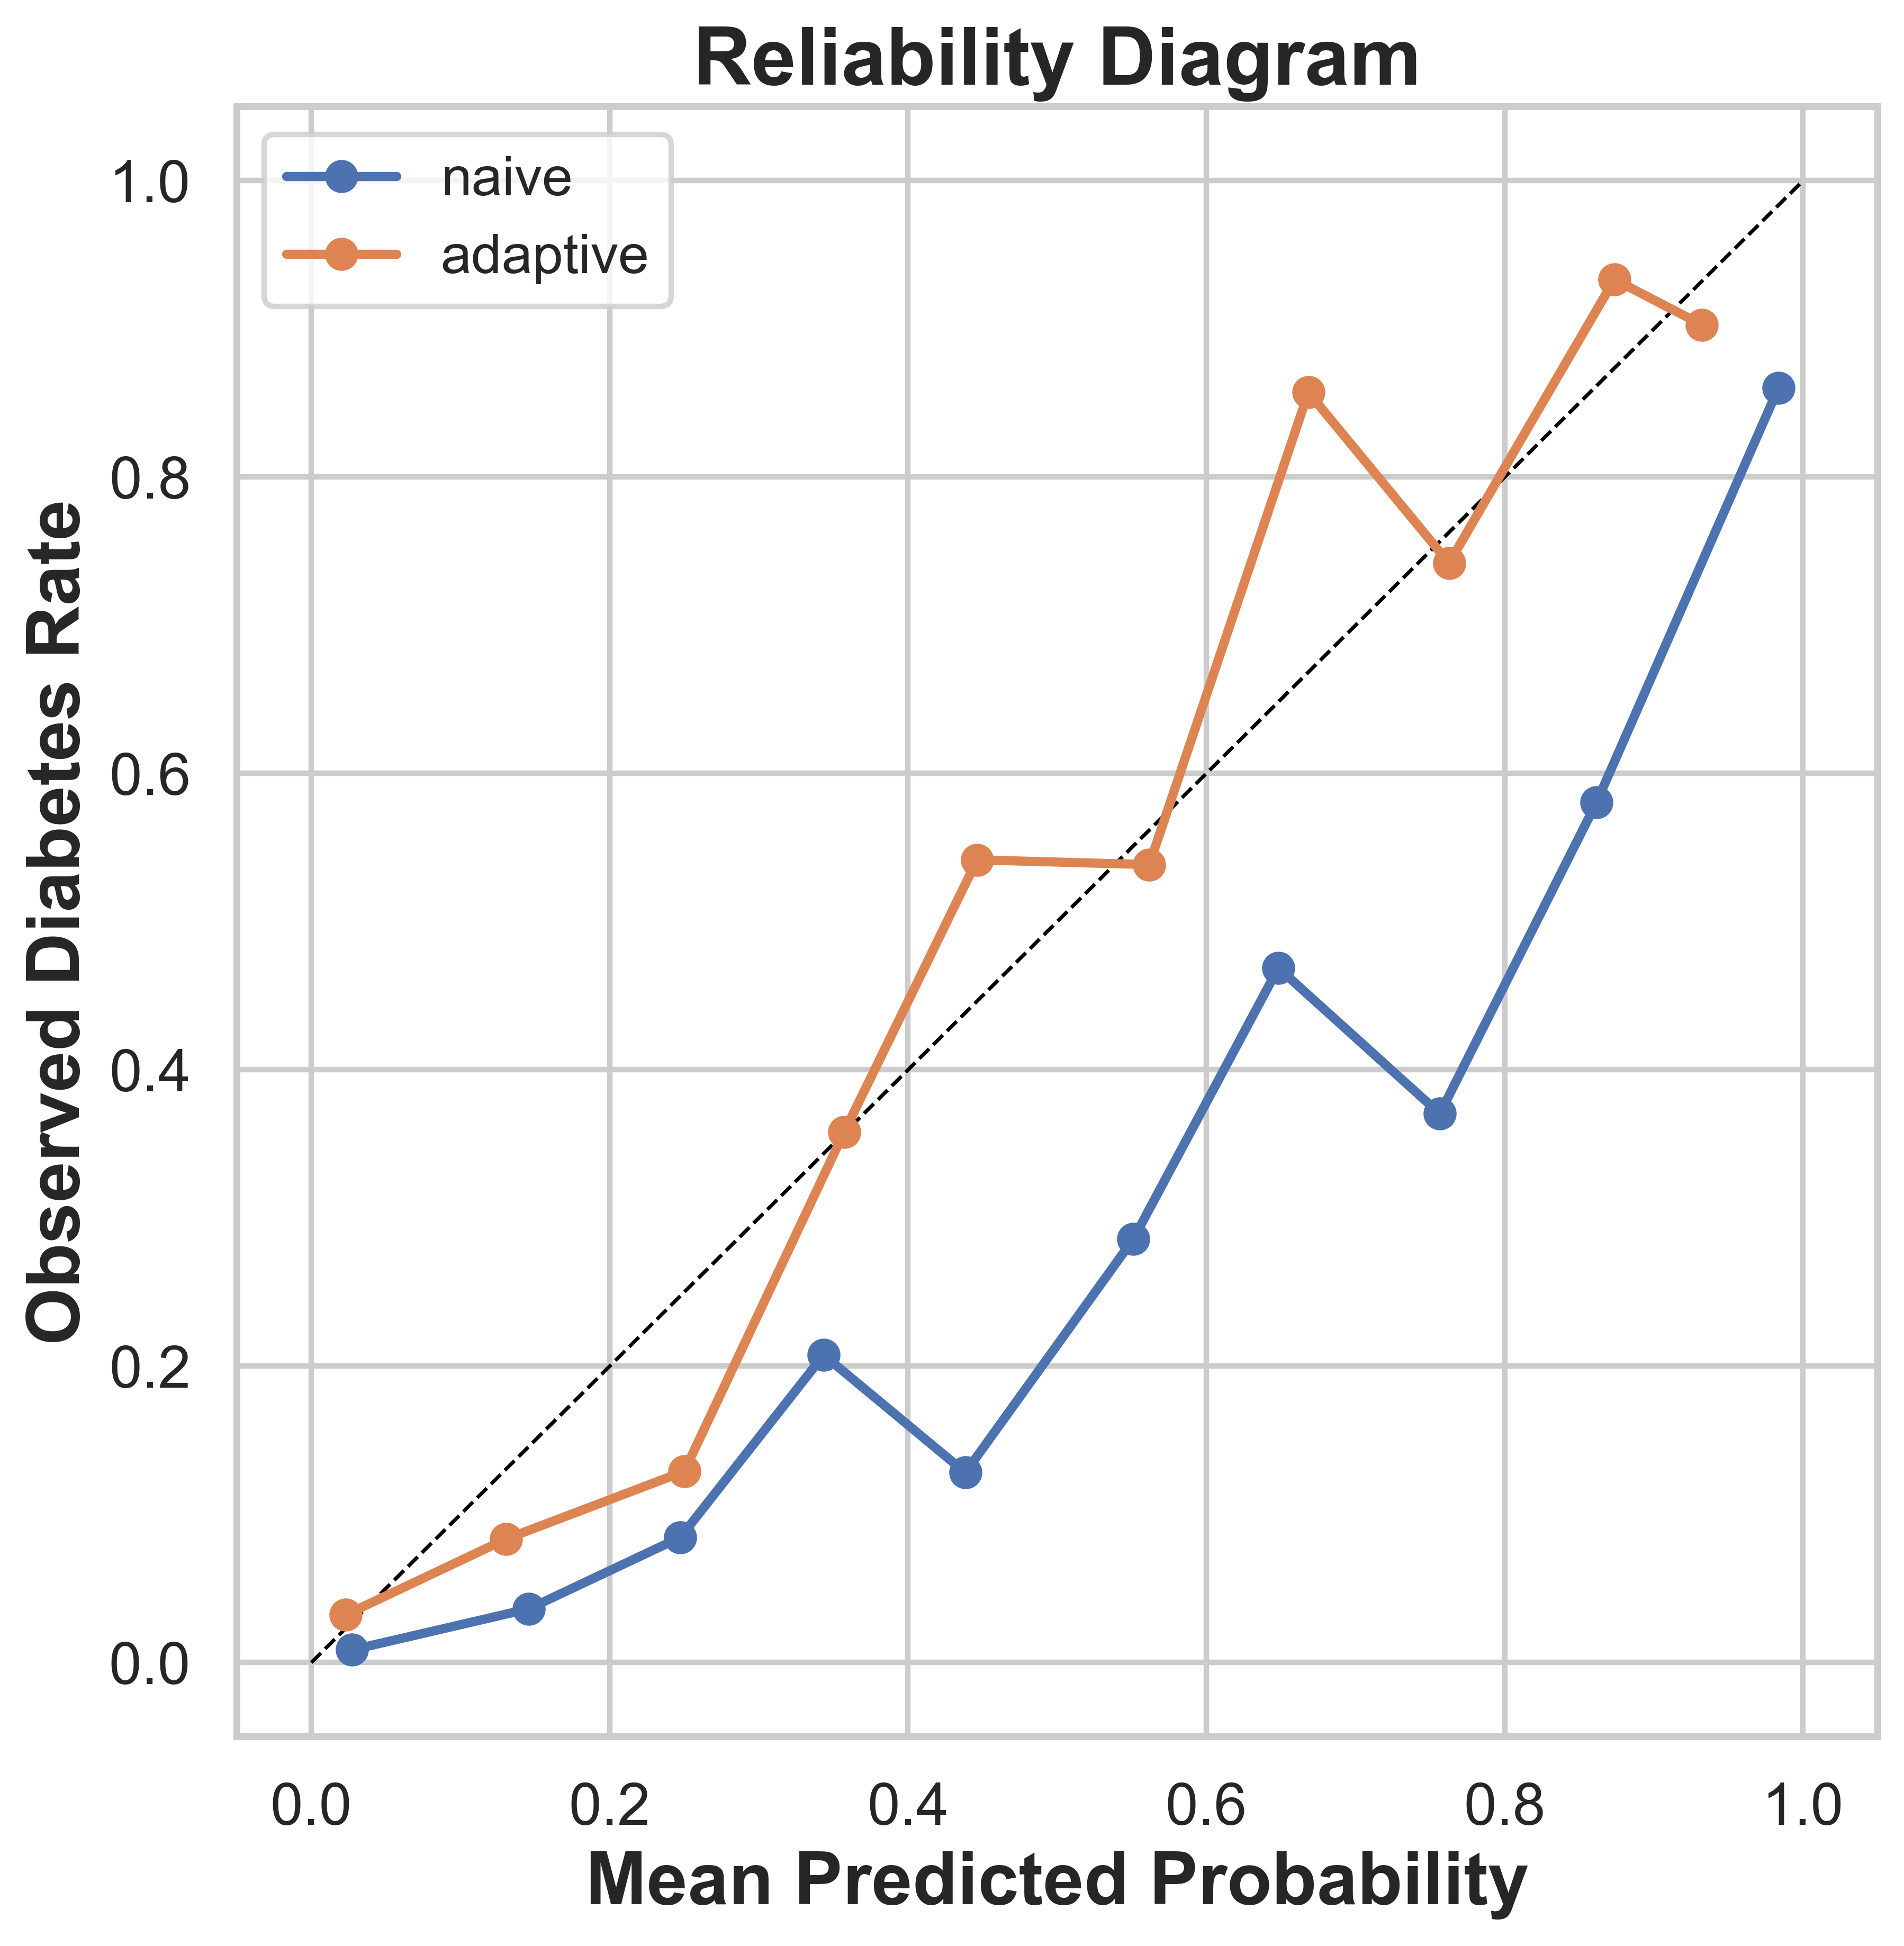
\includegraphics[width=\linewidth]{figure_reliability_logistic_regression_nhanes.png}
    \caption{Logistic regression}
\end{subfigure}
\hfill
\begin{subfigure}{0.48\linewidth}
    \centering
    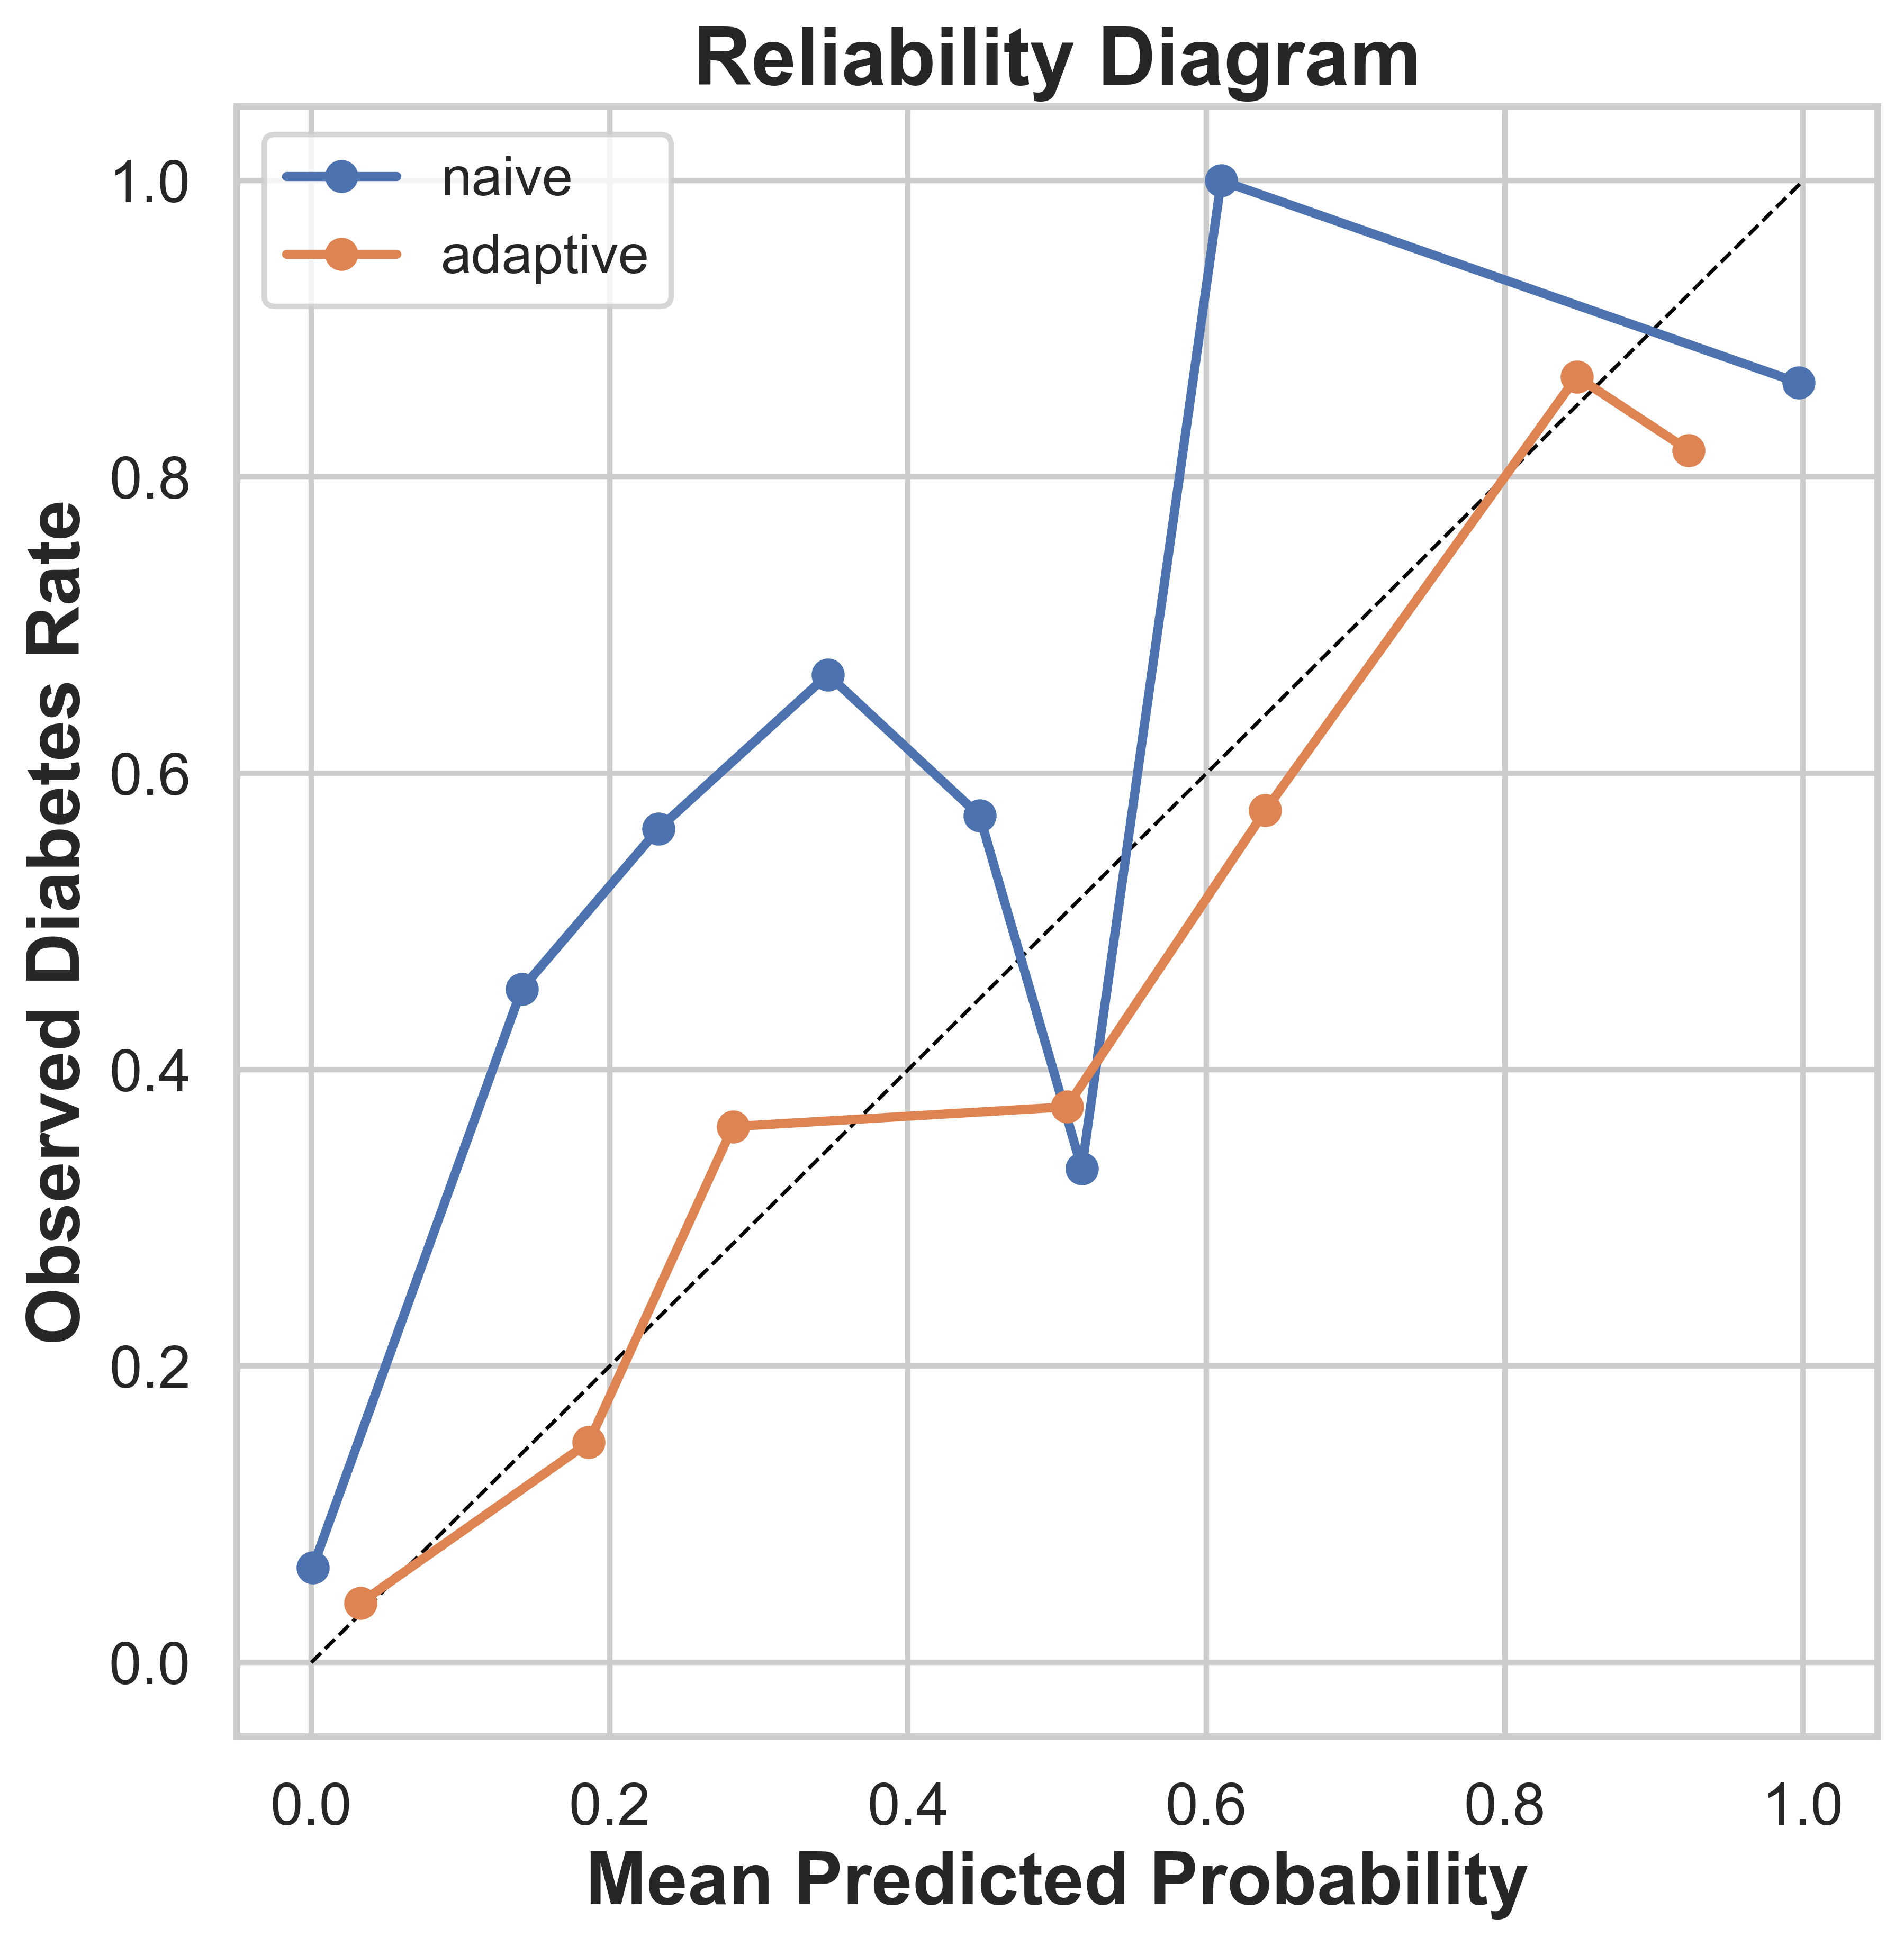
\includegraphics[width=\linewidth]{figure_reliability_xgboost_nhanes.png}
    \caption{XGBoost}
\end{subfigure}
\caption{NHANES reliability diagrams before and after adaptive calibration.}
\label{fig:reliability}
\end{figure}

\begin{table}[H]
\centering
\caption{Bootstrap confidence intervals for the top TRS setting: NHANES, extended random forest, adaptive isotonic calibration.}
\label{tab:bootstrap}
\begin{tabular}{lrrr}
\toprule
Metric & Estimate & 95\% CI lower & 95\% CI upper \\
\midrule
ROC-AUC & 0.924 & 0.904 & 0.943 \\
Brier score & 0.073 & 0.064 & 0.083 \\
ECE & 0.023 & 0.013 & 0.034 \\
Coverage & 0.904 & 0.890 & 0.918 \\
\bottomrule
\end{tabular}
\end{table}

\subsection{Fairness and Subgroup Reliability}
Subgroup reliability gaps remained meaningful. In NHANES, the lowest reliability-gap settings were random forest settings, with reliability gap around 0.197--0.218. In Pima, some XGBoost settings had smaller reliability gaps, but these did not solve the overall coverage failure. This shows why TRS must be interpreted together with raw coverage and class-wise coverage.

\begin{table}[H]
\centering
\caption{Lowest reliability-gap settings by target dataset.}
\label{tab:fairness}
\begin{adjustbox}{width=\textwidth}
\begin{tabular}{llllrrr}
\toprule
Target & Feature set & Model & Scenario & Equal opportunity diff. & Calibration diff. & Reliability gap \\
\midrule
NHANES & Routine clinical & Random forest & Fixed recalibration & 0.197 & 0.060 & 0.197 \\
NHANES & Routine clinical & Random forest & Naive transfer & 0.197 & 0.060 & 0.197 \\
NHANES & Extended transport & Random forest & Adaptive isotonic & 0.215 & 0.083 & 0.215 \\
Pima & Extended transport & XGBoost & Fixed temperature & 0.000 & 0.061 & 0.061 \\
Pima & Routine clinical & XGBoost & Fixed temperature & 0.000 & 0.070 & 0.070 \\
Pima & Screening & CatBoost & Naive transfer & 0.000 & 0.060 & 0.168 \\
\bottomrule
\end{tabular}
\end{adjustbox}
\end{table}

\section{Discussion}
\subsection{Principal Findings}
The main finding is that transport reliability depends strongly on the target dataset. NHANES showed promising results. The best external discrimination was high, adaptive calibration improved calibration error, and ATCP reached near-nominal 90\% marginal coverage in the best settings. Pima did not show the same reliability. Although discrimination remained moderate, conformal coverage was far below the 90\% target.

\subsection{Why NHANES Was More Reliable}
NHANES is shifted from the source data, but it still contains several comparable clinical variables such as age, BMI, glucose, and HbA1c. These variables allow meaningful source-to-target transport after calibration. The best NHANES models were routine or extended clinical models, confirming the value of laboratory features.

\subsection{Why Pima Failed as a Reliability Target}
Pima differs more strongly in prevalence, demographic structure, and feature availability. Several variables used by the source model are absent or not comparable in Pima. Under this severe shift, adaptive calibration improved some probability metrics but did not restore conformal reliability. The Pima result should therefore be interpreted as a stress-test failure rather than a successful deployment case.

\subsection{Clinical and Methodological Implications}
This study supports a practical workflow for clinical model transport. First, measure dataset shift. Second, evaluate discrimination and calibration externally. Third, recalibrate probabilities using target data when available. Fourth, check conformal coverage in the target population. Fifth, evaluate subgroup reliability. If coverage fails, the model should not be presented as deployment-ready.

\subsection{Limitations}
This study used public datasets with different outcome definitions. NHANES diabetes status was based on self-reported clinician diagnosis, while the source dataset outcome definition is dataset-specific. Pima has limited demographic variables and lacks several source predictors. Model hyperparameters were fixed initial settings rather than exhaustive tuning. TRS used equal weights and should be validated further. Finally, target calibration used labeled target subsets; in settings without such labels, adaptive recalibration would require a different deployment strategy.

\section{Conclusion}
This study evaluated adaptive transport calibration for diabetes classification across source, external validation, and stress-test datasets. All five planned model families were included. Internal source performance was strong, with CatBoost and XGBoost achieving ROC-AUC around 0.977. NHANES external validation was promising: adaptive calibration improved probability reliability, and ATCP achieved near-nominal 90\% marginal coverage in the best settings. Pima exposed the limits of the method: best 90\% ATCP coverage was only 0.747. The final conclusion is that adaptive calibration and ATCP can improve reliability under moderate dataset shift, but severe shift can still break uncertainty guarantees. Reliable clinical deployment requires explicit shift measurement, target calibration, conformal validation, and subgroup reliability reporting.

\section*{Data and Reproducibility}
All reported results were generated from the corrected full five-model experiment. The output folder contains harmonized data files, result tables, models, logs, and 500-dpi figures. The key result tables used in this manuscript are \texttt{table\_02} through \texttt{table\_13} in the experiment output directory.

\section*{Acknowledgment}
Author details, institution, and funding information should be added before submission.

\bibliographystyle{plain}
\bibliography{ref}

\end{document}
